\documentclass[]{book}
\usepackage{lmodern}
\usepackage{amssymb,amsmath}
\usepackage{ifxetex,ifluatex}
\usepackage{fixltx2e} % provides \textsubscript
\ifnum 0\ifxetex 1\fi\ifluatex 1\fi=0 % if pdftex
  \usepackage[T1]{fontenc}
  \usepackage[utf8]{inputenc}
\else % if luatex or xelatex
  \ifxetex
    \usepackage{mathspec}
  \else
    \usepackage{fontspec}
  \fi
  \defaultfontfeatures{Ligatures=TeX,Scale=MatchLowercase}
\fi
% use upquote if available, for straight quotes in verbatim environments
\IfFileExists{upquote.sty}{\usepackage{upquote}}{}
% use microtype if available
\IfFileExists{microtype.sty}{%
\usepackage{microtype}
\UseMicrotypeSet[protrusion]{basicmath} % disable protrusion for tt fonts
}{}
\usepackage{hyperref}
\hypersetup{unicode=true,
            pdftitle={OMG},
            pdfauthor={NVP},
            pdfborder={0 0 0},
            breaklinks=true}
\urlstyle{same}  % don't use monospace font for urls
\usepackage{natbib}
\bibliographystyle{plainnat}
\usepackage{color}
\usepackage{fancyvrb}
\newcommand{\VerbBar}{|}
\newcommand{\VERB}{\Verb[commandchars=\\\{\}]}
\DefineVerbatimEnvironment{Highlighting}{Verbatim}{commandchars=\\\{\}}
% Add ',fontsize=\small' for more characters per line
\usepackage{framed}
\definecolor{shadecolor}{RGB}{248,248,248}
\newenvironment{Shaded}{\begin{snugshade}}{\end{snugshade}}
\newcommand{\AlertTok}[1]{\textcolor[rgb]{0.94,0.16,0.16}{#1}}
\newcommand{\AnnotationTok}[1]{\textcolor[rgb]{0.56,0.35,0.01}{\textbf{\textit{#1}}}}
\newcommand{\AttributeTok}[1]{\textcolor[rgb]{0.77,0.63,0.00}{#1}}
\newcommand{\BaseNTok}[1]{\textcolor[rgb]{0.00,0.00,0.81}{#1}}
\newcommand{\BuiltInTok}[1]{#1}
\newcommand{\CharTok}[1]{\textcolor[rgb]{0.31,0.60,0.02}{#1}}
\newcommand{\CommentTok}[1]{\textcolor[rgb]{0.56,0.35,0.01}{\textit{#1}}}
\newcommand{\CommentVarTok}[1]{\textcolor[rgb]{0.56,0.35,0.01}{\textbf{\textit{#1}}}}
\newcommand{\ConstantTok}[1]{\textcolor[rgb]{0.00,0.00,0.00}{#1}}
\newcommand{\ControlFlowTok}[1]{\textcolor[rgb]{0.13,0.29,0.53}{\textbf{#1}}}
\newcommand{\DataTypeTok}[1]{\textcolor[rgb]{0.13,0.29,0.53}{#1}}
\newcommand{\DecValTok}[1]{\textcolor[rgb]{0.00,0.00,0.81}{#1}}
\newcommand{\DocumentationTok}[1]{\textcolor[rgb]{0.56,0.35,0.01}{\textbf{\textit{#1}}}}
\newcommand{\ErrorTok}[1]{\textcolor[rgb]{0.64,0.00,0.00}{\textbf{#1}}}
\newcommand{\ExtensionTok}[1]{#1}
\newcommand{\FloatTok}[1]{\textcolor[rgb]{0.00,0.00,0.81}{#1}}
\newcommand{\FunctionTok}[1]{\textcolor[rgb]{0.00,0.00,0.00}{#1}}
\newcommand{\ImportTok}[1]{#1}
\newcommand{\InformationTok}[1]{\textcolor[rgb]{0.56,0.35,0.01}{\textbf{\textit{#1}}}}
\newcommand{\KeywordTok}[1]{\textcolor[rgb]{0.13,0.29,0.53}{\textbf{#1}}}
\newcommand{\NormalTok}[1]{#1}
\newcommand{\OperatorTok}[1]{\textcolor[rgb]{0.81,0.36,0.00}{\textbf{#1}}}
\newcommand{\OtherTok}[1]{\textcolor[rgb]{0.56,0.35,0.01}{#1}}
\newcommand{\PreprocessorTok}[1]{\textcolor[rgb]{0.56,0.35,0.01}{\textit{#1}}}
\newcommand{\RegionMarkerTok}[1]{#1}
\newcommand{\SpecialCharTok}[1]{\textcolor[rgb]{0.00,0.00,0.00}{#1}}
\newcommand{\SpecialStringTok}[1]{\textcolor[rgb]{0.31,0.60,0.02}{#1}}
\newcommand{\StringTok}[1]{\textcolor[rgb]{0.31,0.60,0.02}{#1}}
\newcommand{\VariableTok}[1]{\textcolor[rgb]{0.00,0.00,0.00}{#1}}
\newcommand{\VerbatimStringTok}[1]{\textcolor[rgb]{0.31,0.60,0.02}{#1}}
\newcommand{\WarningTok}[1]{\textcolor[rgb]{0.56,0.35,0.01}{\textbf{\textit{#1}}}}
\usepackage{longtable,booktabs}
\usepackage{graphicx}
% grffile has become a legacy package: https://ctan.org/pkg/grffile
\IfFileExists{grffile.sty}{%
\usepackage{grffile}
}{}
\makeatletter
\def\maxwidth{\ifdim\Gin@nat@width>\linewidth\linewidth\else\Gin@nat@width\fi}
\def\maxheight{\ifdim\Gin@nat@height>\textheight\textheight\else\Gin@nat@height\fi}
\makeatother
% Scale images if necessary, so that they will not overflow the page
% margins by default, and it is still possible to overwrite the defaults
% using explicit options in \includegraphics[width, height, ...]{}
\setkeys{Gin}{width=\maxwidth,height=\maxheight,keepaspectratio}
\IfFileExists{parskip.sty}{%
\usepackage{parskip}
}{% else
\setlength{\parindent}{0pt}
\setlength{\parskip}{6pt plus 2pt minus 1pt}
}
\setlength{\emergencystretch}{3em}  % prevent overfull lines
\providecommand{\tightlist}{%
  \setlength{\itemsep}{0pt}\setlength{\parskip}{0pt}}
\setcounter{secnumdepth}{5}
% Redefines (sub)paragraphs to behave more like sections
\ifx\paragraph\undefined\else
\let\oldparagraph\paragraph
\renewcommand{\paragraph}[1]{\oldparagraph{#1}\mbox{}}
\fi
\ifx\subparagraph\undefined\else
\let\oldsubparagraph\subparagraph
\renewcommand{\subparagraph}[1]{\oldsubparagraph{#1}\mbox{}}
\fi

%%% Use protect on footnotes to avoid problems with footnotes in titles
\let\rmarkdownfootnote\footnote%
\def\footnote{\protect\rmarkdownfootnote}

%%% Change title format to be more compact
\usepackage{titling}

% Create subtitle command for use in maketitle
\providecommand{\subtitle}[1]{
  \posttitle{
    \begin{center}\large#1\end{center}
    }
}

\setlength{\droptitle}{-2em}

  \title{OMG}
    \pretitle{\vspace{\droptitle}\centering\huge}
  \posttitle{\par}
  \subtitle{The OCC Knowledge Base}
  \author{NVP}
    \preauthor{\centering\large\emph}
  \postauthor{\par}
      \predate{\centering\large\emph}
  \postdate{\par}
    \date{2020-03-19}

\usepackage{booktabs}
\usepackage{amsthm}
\makeatletter
\def\thm@space@setup{%
  \thm@preskip=8pt plus 2pt minus 4pt
  \thm@postskip=\thm@preskip
}
\makeatother
\usepackage{fontspec}
\setmainfont{Calibri}

\begin{document}
\maketitle

{
\setcounter{tocdepth}{1}
\tableofcontents
}
\hypertarget{preface}{%
\chapter*{Preface}\label{preface}}
\addcontentsline{toc}{chapter}{Preface}

\includegraphics{images/OCC_Diurnal_Suite_Recovery_CJS.jpg}

Welcome to the online knowledge base of the OCC Team. This started as the OCC Mission Guide, a reference manual to help consolidate best practices for conducting OCC team operations at sea. As of 2020, it has evolved into an online living book, written in R Markdown and compiled into book with \href{https://bookdown.org/yihui/bookdown/}{bookdown},published via \href{https://pages.github.com/}{GitHub Pages}. The current live version of the book that you can bookmark is \href{https://npomeroy.github.io/OMG/}{here}. All OCC team members are encouraged to not only use it as a resource but help it grow by adding and editing content as OCC projects, methods and missions continue to change and grow. Anyone may suggest edits to the contents of the OMG by forking the OMG repository from \href{https://github.com/npomeroy/OMG}{Noah via GitHub}, pushing any changes back to GitHub, after which they may be approved for incorporation into the master copy of the OMG.

Once you have forked the repo onto your local machine, the HTML version of the OMG may be accessed offline by simply opening the index.html file in the folder ``OMG/docs'' A .PDF file of the book is also generated every time the book is built, that also ends up in the ``OMG/docs'' folder.

\hypertarget{how-to-edit-this-book}{%
\section*{How to Edit this Book}\label{how-to-edit-this-book}}
\addcontentsline{toc}{section}{How to Edit this Book}

\begin{enumerate}
\def\labelenumi{\arabic{enumi}.}
\tightlist
\item
  Fork the repo from \href{https://github.com/npomeroy/OMG}{Noah via GitHub}.
\item
  Edit any existing chapter by simply editing its .Rmd file in R studio or create a new chapter by creating a new .Rmd file in the root OMG folder. Build the book to see your edits in the form of the built book.
\item
  Commit your changes via GitHub Desktop (or via R if you have setup GitHub to play nicely with R.)
\item
  In GitHub, open a Pull Request to have your edits considered for integration into the master branch.
\end{enumerate}

\textbf{The Best How to Guide for Authoring Books with R Markdown} is written by Yihui Xie and is found right \href{https://bookdown.org/yihui/bookdown/}{here}

If you need some tips for your R Markdown formatting, \href{https://rmarkdown.rstudio.com/lesson-15.html}{this cheat sheet is great.}

\hypertarget{cruise_prep}{%
\chapter{Preparing for a Research Cruise}\label{cruise_prep}}

\includegraphics{images/Sette_Big_Island_2010_Pomeroy.jpg}

\hypertarget{determine-goals}{%
\section{Determine Goals}\label{determine-goals}}

Determine the team's goals in the region the research cruise is scheduled to visit. Identify all planned retreivals, deployments and specialty projects (such as the diel suite), and the number of days, staff, and boats needed to accomplish these goals.

\hypertarget{htmlwidget-eedfb1102584adc6687d}{}

\hypertarget{spatial-data-preparation}{%
\section{Spatial Data Preparation}\label{spatial-data-preparation}}

\begin{itemize}
\tightlist
\item
  Create a single .kml file that includes all planned instrument retrievals and any planned additional deployments and other necessary points (collectively all called ``planning points''. .kml files are more agile than ArcGIS files; they are easier to use in Google Earth for day to day planning.
\item
  Create an ArcGIS map project that contains the locations of all planning points.
\end{itemize}

\hypertarget{garmin-78-handheld-gps-preparation}{%
\section{Garmin 78 Handheld GPS Preparation}\label{garmin-78-handheld-gps-preparation}}

\begin{itemize}
\tightlist
\item
  Ensure each handheld unit is setup properly

  \begin{itemize}
  \tightlist
  \item
    Time to UTC
  \item
    LAT and LONG in decimal degrees
  \end{itemize}
\item
  Test each handheld GPS to be taken on the cruise prior to sailing: take it outside and ensure that it collects waypoints.
\item
  Upload planning points to both the primary and secondary GPS units.
\end{itemize}

\hypertarget{datasheet-preparation}{%
\section{Datasheet Preparation}\label{datasheet-preparation}}

\begin{itemize}
\item
  We should make some new field datasheets before MARAMP2020 given the NEW FANCY Oracle DB!!!!!!!!
\item
  Prepare Field Data Binders

  \begin{itemize}
  \tightlist
  \item
    Print enough data sheets for all activities, including mooring, CAU, CTD/H2O for the OCC team in addition to enough CTD/H20 data sheets for any other team on CTD/H20 Ops.
  \item
    Attach sharp pencils to field binders
  \end{itemize}
\end{itemize}

\hypertarget{software-needed-at-sea}{%
\section{Software Needed at Sea}\label{software-needed-at-sea}}

\begin{longtable}[]{@{}llllll@{}}
\toprule
\begin{minipage}[b]{0.14\columnwidth}\raggedright
Software\strut
\end{minipage} & \begin{minipage}[b]{0.06\columnwidth}\raggedright
Team Lead Only\strut
\end{minipage} & \begin{minipage}[b]{0.07\columnwidth}\raggedright
Manufacturer\strut
\end{minipage} & \begin{minipage}[b]{0.18\columnwidth}\raggedright
Needed For\strut
\end{minipage} & \begin{minipage}[b]{0.08\columnwidth}\raggedright
Instrument\strut
\end{minipage} & \begin{minipage}[b]{0.30\columnwidth}\raggedright
Download Location\strut
\end{minipage}\tabularnewline
\midrule
\endhead
\begin{minipage}[t]{0.14\columnwidth}\raggedright
ARCMap\strut
\end{minipage} & \begin{minipage}[t]{0.06\columnwidth}\raggedright
x\strut
\end{minipage} & \begin{minipage}[t]{0.07\columnwidth}\raggedright
ESRI\strut
\end{minipage} & \begin{minipage}[t]{0.18\columnwidth}\raggedright
planning operations and generating maps\strut
\end{minipage} & \begin{minipage}[t]{0.08\columnwidth}\raggedright
NA\strut
\end{minipage} & \begin{minipage}[t]{0.30\columnwidth}\raggedright
see Tomoko\strut
\end{minipage}\tabularnewline
\begin{minipage}[t]{0.14\columnwidth}\raggedright
Google Earth\strut
\end{minipage} & \begin{minipage}[t]{0.06\columnwidth}\raggedright
\strut
\end{minipage} & \begin{minipage}[t]{0.07\columnwidth}\raggedright
Google\strut
\end{minipage} & \begin{minipage}[t]{0.18\columnwidth}\raggedright
planning operations\strut
\end{minipage} & \begin{minipage}[t]{0.08\columnwidth}\raggedright
NA\strut
\end{minipage} & \begin{minipage}[t]{0.30\columnwidth}\raggedright
\strut
\end{minipage}\tabularnewline
\begin{minipage}[t]{0.14\columnwidth}\raggedright
Keyspan USA Software\strut
\end{minipage} & \begin{minipage}[t]{0.06\columnwidth}\raggedright
\strut
\end{minipage} & \begin{minipage}[t]{0.07\columnwidth}\raggedright
Keyspan\strut
\end{minipage} & \begin{minipage}[t]{0.18\columnwidth}\raggedright
serial to USB adapter cable\strut
\end{minipage} & \begin{minipage}[t]{0.08\columnwidth}\raggedright
GPS\strut
\end{minipage} & \begin{minipage}[t]{0.30\columnwidth}\raggedright
\url{https://www.tripplite.com/support/USA19HS}\strut
\end{minipage}\tabularnewline
\begin{minipage}[t]{0.14\columnwidth}\raggedright
Microsoft Access 2010\strut
\end{minipage} & \begin{minipage}[t]{0.06\columnwidth}\raggedright
\strut
\end{minipage} & \begin{minipage}[t]{0.07\columnwidth}\raggedright
Microsoft\strut
\end{minipage} & \begin{minipage}[t]{0.18\columnwidth}\raggedright
mooring and CTD databases\strut
\end{minipage} & \begin{minipage}[t]{0.08\columnwidth}\raggedright
NA\strut
\end{minipage} & \begin{minipage}[t]{0.30\columnwidth}\raggedright
request from ITS\strut
\end{minipage}\tabularnewline
\begin{minipage}[t]{0.14\columnwidth}\raggedright
Excel\strut
\end{minipage} & \begin{minipage}[t]{0.06\columnwidth}\raggedright
\strut
\end{minipage} & \begin{minipage}[t]{0.07\columnwidth}\raggedright
Microsoft\strut
\end{minipage} & \begin{minipage}[t]{0.18\columnwidth}\raggedright
spreadsheets\strut
\end{minipage} & \begin{minipage}[t]{0.08\columnwidth}\raggedright
NA\strut
\end{minipage} & \begin{minipage}[t]{0.30\columnwidth}\raggedright
you must have this already\strut
\end{minipage}\tabularnewline
\begin{minipage}[t]{0.14\columnwidth}\raggedright
DNR Garmin\strut
\end{minipage} & \begin{minipage}[t]{0.06\columnwidth}\raggedright
\strut
\end{minipage} & \begin{minipage}[t]{0.07\columnwidth}\raggedright
Minnesota DNR\strut
\end{minipage} & \begin{minipage}[t]{0.18\columnwidth}\raggedright
download of GPS Waypoints\strut
\end{minipage} & \begin{minipage}[t]{0.08\columnwidth}\raggedright
GPS\strut
\end{minipage} & \begin{minipage}[t]{0.30\columnwidth}\raggedright
\url{http://www.dnr.state.mn.us/mis/gis/tools/arcview/extensions/DNRGarmin/DNRGarmin.html}\strut
\end{minipage}\tabularnewline
\begin{minipage}[t]{0.14\columnwidth}\raggedright
DNR GPS\strut
\end{minipage} & \begin{minipage}[t]{0.06\columnwidth}\raggedright
\strut
\end{minipage} & \begin{minipage}[t]{0.07\columnwidth}\raggedright
Minnesota DNR\strut
\end{minipage} & \begin{minipage}[t]{0.18\columnwidth}\raggedright
upload of GPS planning points from Google Earth\strut
\end{minipage} & \begin{minipage}[t]{0.08\columnwidth}\raggedright
GPS\strut
\end{minipage} & \begin{minipage}[t]{0.30\columnwidth}\raggedright
\url{http://www.dnr.state.mn.us/mis/gis/DNRGPS/DNRGPS.html}\strut
\end{minipage}\tabularnewline
\begin{minipage}[t]{0.14\columnwidth}\raggedright
Aquadopp Software - AquaPro v1.37.08\strut
\end{minipage} & \begin{minipage}[t]{0.06\columnwidth}\raggedright
\strut
\end{minipage} & \begin{minipage}[t]{0.07\columnwidth}\raggedright
Nortek\strut
\end{minipage} & \begin{minipage}[t]{0.18\columnwidth}\raggedright
instrument interface\strut
\end{minipage} & \begin{minipage}[t]{0.08\columnwidth}\raggedright
Aquadopp ADCP\strut
\end{minipage} & \begin{minipage}[t]{0.30\columnwidth}\raggedright
\url{http://www.nortek-as.com/en/support/software}\strut
\end{minipage}\tabularnewline
\begin{minipage}[t]{0.14\columnwidth}\raggedright
SoundTrap Host Software Version 2.0.9.x\strut
\end{minipage} & \begin{minipage}[t]{0.06\columnwidth}\raggedright
x\strut
\end{minipage} & \begin{minipage}[t]{0.07\columnwidth}\raggedright
Ocean Instruments\strut
\end{minipage} & \begin{minipage}[t]{0.18\columnwidth}\raggedright
instrument interface\strut
\end{minipage} & \begin{minipage}[t]{0.08\columnwidth}\raggedright
Sound Trap\strut
\end{minipage} & \begin{minipage}[t]{0.30\columnwidth}\raggedright
\url{http://www.oceaninstruments.co.nz/downloads/}\strut
\end{minipage}\tabularnewline
\begin{minipage}[t]{0.14\columnwidth}\raggedright
Basic Stamp Editor\strut
\end{minipage} & \begin{minipage}[t]{0.06\columnwidth}\raggedright
\strut
\end{minipage} & \begin{minipage}[t]{0.07\columnwidth}\raggedright
Paralax Inc.\strut
\end{minipage} & \begin{minipage}[t]{0.18\columnwidth}\raggedright
instrument interface\strut
\end{minipage} & \begin{minipage}[t]{0.08\columnwidth}\raggedright
PUC\strut
\end{minipage} & \begin{minipage}[t]{0.30\columnwidth}\raggedright
\url{https://www.parallax.com/downloads/basic-stamp-editor-software-windows}\strut
\end{minipage}\tabularnewline
\begin{minipage}[t]{0.14\columnwidth}\raggedright
Python 2.51\strut
\end{minipage} & \begin{minipage}[t]{0.06\columnwidth}\raggedright
\strut
\end{minipage} & \begin{minipage}[t]{0.07\columnwidth}\raggedright
Python\strut
\end{minipage} & \begin{minipage}[t]{0.18\columnwidth}\raggedright
scripts that are part of mooring and CTD databases\strut
\end{minipage} & \begin{minipage}[t]{0.08\columnwidth}\raggedright
NA\strut
\end{minipage} & \begin{minipage}[t]{0.30\columnwidth}\raggedright
\url{https://www.python.org/download/releases/2.5.1/}\strut
\end{minipage}\tabularnewline
\begin{minipage}[t]{0.14\columnwidth}\raggedright
SeaFETCOM 2\strut
\end{minipage} & \begin{minipage}[t]{0.06\columnwidth}\raggedright
\strut
\end{minipage} & \begin{minipage}[t]{0.07\columnwidth}\raggedright
Satlantic\strut
\end{minipage} & \begin{minipage}[t]{0.18\columnwidth}\raggedright
instrument interface\strut
\end{minipage} & \begin{minipage}[t]{0.08\columnwidth}\raggedright
SeaFet\strut
\end{minipage} & \begin{minipage}[t]{0.30\columnwidth}\raggedright
\url{http://satlantic.com/seafetcom}\strut
\end{minipage}\tabularnewline
\begin{minipage}[t]{0.14\columnwidth}\raggedright
Seaterm 1.59\strut
\end{minipage} & \begin{minipage}[t]{0.06\columnwidth}\raggedright
\strut
\end{minipage} & \begin{minipage}[t]{0.07\columnwidth}\raggedright
SeaBird\strut
\end{minipage} & \begin{minipage}[t]{0.18\columnwidth}\raggedright
instrument interface\strut
\end{minipage} & \begin{minipage}[t]{0.08\columnwidth}\raggedright
SBE39, SBE19, SBE19+\strut
\end{minipage} & \begin{minipage}[t]{0.30\columnwidth}\raggedright
\url{http://www.seabird.com/software/software}\strut
\end{minipage}\tabularnewline
\begin{minipage}[t]{0.14\columnwidth}\raggedright
Seaterm V2\strut
\end{minipage} & \begin{minipage}[t]{0.06\columnwidth}\raggedright
\strut
\end{minipage} & \begin{minipage}[t]{0.07\columnwidth}\raggedright
SeaBird\strut
\end{minipage} & \begin{minipage}[t]{0.18\columnwidth}\raggedright
instrument interface\strut
\end{minipage} & \begin{minipage}[t]{0.08\columnwidth}\raggedright
sbe19+ V2, SBE56\strut
\end{minipage} & \begin{minipage}[t]{0.30\columnwidth}\raggedright
\url{http://www.seabird.com/software/software}\strut
\end{minipage}\tabularnewline
\begin{minipage}[t]{0.14\columnwidth}\raggedright
SBE Data Processing\strut
\end{minipage} & \begin{minipage}[t]{0.06\columnwidth}\raggedright
\strut
\end{minipage} & \begin{minipage}[t]{0.07\columnwidth}\raggedright
SeaBird\strut
\end{minipage} & \begin{minipage}[t]{0.18\columnwidth}\raggedright
CTD cast processing\strut
\end{minipage} & \begin{minipage}[t]{0.08\columnwidth}\raggedright
SBE CTDs\strut
\end{minipage} & \begin{minipage}[t]{0.30\columnwidth}\raggedright
\url{https://www.seabird.com/software-updates}\strut
\end{minipage}\tabularnewline
\begin{minipage}[t]{0.14\columnwidth}\raggedright
R and R Studio for STR processing\strut
\end{minipage} & \begin{minipage}[t]{0.06\columnwidth}\raggedright
\strut
\end{minipage} & \begin{minipage}[t]{0.07\columnwidth}\raggedright
R Studio\strut
\end{minipage} & \begin{minipage}[t]{0.18\columnwidth}\raggedright
data processing\strut
\end{minipage} & \begin{minipage}[t]{0.08\columnwidth}\raggedright
all\strut
\end{minipage} & \begin{minipage}[t]{0.30\columnwidth}\raggedright
\url{https://www.rstudio.com/products/rstudio/download/}\strut
\end{minipage}\tabularnewline
\begin{minipage}[t]{0.14\columnwidth}\raggedright
Ruskin\strut
\end{minipage} & \begin{minipage}[t]{0.06\columnwidth}\raggedright
\strut
\end{minipage} & \begin{minipage}[t]{0.07\columnwidth}\raggedright
RBR\strut
\end{minipage} & \begin{minipage}[t]{0.18\columnwidth}\raggedright
STR, PAR, DO\strut
\end{minipage} & \begin{minipage}[t]{0.08\columnwidth}\raggedright
RBR Solo\strut
\end{minipage} & \begin{minipage}[t]{0.30\columnwidth}\raggedright
\url{https://rbr-global.com/products/software}\strut
\end{minipage}\tabularnewline
\bottomrule
\end{longtable}

\hypertarget{water}{%
\chapter{CTD and DIC Water Sampling Field Guide}\label{water}}

If available hands on deck and conditions allow, please conduct the CTD downcast and the water sample collection simultaneously.

\hypertarget{waypoint-and-metadata-collection}{%
\section{Waypoint and metadata collection}\label{waypoint-and-metadata-collection}}

Use the OCC provided GPS unit to collect a waypoint when the CTD downcast begins. Record all metadata on provided data sheet.

\hypertarget{ctd-cast}{%
\section{CTD CAST}\label{ctd-cast}}

\begin{enumerate}
\def\labelenumi{\arabic{enumi}.}
\tightlist
\item
  Ensure that the CTD line is connected to the top of the CTD frame by 1 shackles.
\item
  Tie non-CTD end of the CTD line to the boat with a bowline or clip off with carabiner.
\item
  Flake CTD line on deck.
\item
  When the coxswain says the CTD can go over the side, raise the CTD switch to the ``ON'' position, and loudly say, ``ON!'' then lower it over the side until the top of the frame is 1 meter below the surface of the water to begin the 1 minute soaking period, either holding the line or cleating off the line to maintain the CTD at soaking depth.
\item
  After 1 minute soak, ask the coxswain for the current depth so you know how far you can lower the CTD without it hitting the bottom (5-10 feet less line than the bottom depth). Un-cleat the CTD line if it was cleated and begin the CTD cast by pulling the CTD frame up until the top ring of the frame emerges from the water, then begin gradually lowering at a consistent rate, hand over hand, until the CTD gets to the target depth (using the markings on the line to estimate depth). Once the target depth is reached, pull the CTD back on board.
\item
  Once the CTD is back on board, lower the switch to ``OFF'', and loudly say ``OFF!''
\end{enumerate}

\hypertarget{water-sample-collection}{%
\section{Water Sample Collection}\label{water-sample-collection}}

\begin{enumerate}
\def\labelenumi{\arabic{enumi}.}
\tightlist
\item
  Prime the Niskin Bottle, ensuring the petcock and the air bleed valve are closed.
\item
  Clip off the boat side of the niskin line to the boat.
\item
  Near the end of the the CTD soaking time, lower the weight and the open Niskin bottle over the side so the top of the Niskin is at 1m depth (surface of water at the BLACK mark drawn on Niskin line).
\item
  Clip the messenger on to the line
\item
  When the CTD begins its downcast, send the messenger to trigger the Niskin to close. Ensure no air bubbles are trapped inside the Niskin and bottle sits vertically in the water column before firing the messenger.
\end{enumerate}

\hypertarget{water-sample-processing}{%
\section{Water sample Processing}\label{water-sample-processing}}

\begin{enumerate}
\def\labelenumi{\arabic{enumi}.}
\tightlist
\item
  Designate roles: bottle filler, mercuric chloride (HgCl2) handler, data recorder. NOTE: Supersaturated mercuric chloride solution is extremely dangerous; use the utmost caution when dealing with the chemical. All personnel working with it are required to wear eye protection. The mercuric chloride handler is also required to where disposable nitrile gloves. In the event of contact with any part of the body, wash the area profusely. If contact is made with eyes, abort operations, rinse continuously with fresh water (or salt if fresh has run out), alert the ship and return ASAP.
\item
  Remove a bottle and its stopper from the storage tote and insert the tygon tubing to the bottom of the bottle. With the tygon tubing attached to the Niskin bottle dispensing nipple, open the Niskin bottle valve and allow for three complete flushings of the bottle to occur before stopping the sample collection (i.e.~start the collection and count how long it takes for the bottle to overflow and then allow that to occur for 2x the required fill time\ldots ie. if the bottle fills in 20 seconds, allow the sample water flow to flush the bottle for 60 seconds). Attention must be given to how the sample water enters the bottle. Care should be given to ensure that smooth water flow into the bottle is maintained and that no bubbles are created during the dispensing of sample. Any bubbles introduced to the sample will alter the pCO2 within the sample water and produce inaccurate DIC results.
\item
  After the appropriate flushing time, shut off the Niskin valve to stop the water flow, while at the same time ensuring the tygon tubing doesn't come off the bottom of the sample bottle. Once the flow is shut off, pinch the tubing and in one motion remove it from the bottle. This ``pinch and remove'' action with the tubing should establish a consistent head-space in all the sample bottles. The meniscus of the sample should be about 1 cm below the neck of the bottle (see picture.)
\end{enumerate}

\includegraphics[width=4.31in]{images/BOD_bottle_headspace}
4.
a. Once the proper head space is established, pipette 200ul of HgCl2 saturated solution into the sample bottle
b. Use the syringe containing vacuum grease to make 3-5 vertical ``stripes'' of grease on a clean, dry stopper. Insert the greased stopper until fully seated in the bottle, then twist until the grease completely seals the bottle contents. The vertical stripes of grease allow for gases to escape the bottle neck while the stopper is being inserted. Having the stopper clean/dry ensures that other than sample water isn't introduced into the bottle. Twisting the stopper, once it has been fully seated into the neck of the bottle, ensures a smooth distribution of grease within the sample bottle's neck and an air tight seal.
c.~Use the rubber band and plastic collar to lock down the stopper inside the bottle. Once secured, softly invert the bottle 1-2x to mix the HgCl2 with the water sampleand secure the sample bottle in the field container.
d.~Complete data sheet including REA Site name or OCC Site Name (if it exists), waypoint name (default), UTC date and time, lat and long, sample depth and DIC bottle \#.

\hypertarget{mercuric-chloride-emergency-procedures}{%
\section{Mercuric Chloride Emergency Procedures}\label{mercuric-chloride-emergency-procedures}}

\begin{itemize}
\tightlist
\item
  Eyes: Irrigate immediately with large quantity of water for at least 15 minutes.
\item
  Skin: Immediately flush with plenty of water for at least 15 minutes. Remove any contaminated clothing.
\item
  Inhalation: Remove to fresh air. If not breathing, give artificial respiration. If breathing is difficult, give oxygen.
\item
  Ingestion: Only induce vomiting if directed to do so by medical personnel.
\item
  The MSDS can be seen from any NOAA Google Account via \href{https://drive.google.com/open?id=12w0Kmi8VVE9n_0A5_BhNVq6l4nMDtM1K}{this google drive link}
\end{itemize}

\hypertarget{mercuric-chloride-safety-data-sheet-sds}{%
\subsection{Mercuric Chloride Safety Data Sheet (SDS)}\label{mercuric-chloride-safety-data-sheet-sds}}

\includegraphics[width=1\textwidth,height=\textheight]{images/Saturated-Mercuric-Chloride-SDS_Page_1.png}
\includegraphics[width=1\textwidth,height=\textheight]{images/Saturated-Mercuric-Chloride-SDS_Page_2.png}
\includegraphics[width=1\textwidth,height=\textheight]{images/Saturated-Mercuric-Chloride-SDS_Page_3.png}
\includegraphics[width=1\textwidth,height=\textheight]{images/Saturated-Mercuric-Chloride-SDS_Page_4.png}
\includegraphics[width=1\textwidth,height=\textheight]{images/Saturated-Mercuric-Chloride-SDS_Page_5.png}
\includegraphics[width=1\textwidth,height=\textheight]{images/Saturated-Mercuric-Chloride-SDS_Page_6.png}
\includegraphics[width=1\textwidth,height=\textheight]{images/Saturated-Mercuric-Chloride-SDS_Page_7.png}
\includegraphics[width=1\textwidth,height=\textheight]{images/Saturated-Mercuric-Chloride-SDS_Page_8.png}
\includegraphics[width=1\textwidth,height=\textheight]{images/Saturated-Mercuric-Chloride-SDS_Page_9.png}
\includegraphics[width=1\textwidth,height=\textheight]{images/Saturated-Mercuric-Chloride-SDS_Page_1.png}

\hypertarget{data_processing}{%
\chapter{Data Processing and the Occ Package}\label{data_processing}}

The \emph{occ} package is uploaded to GitHub and can be downloaded directly in R.

\begin{enumerate}
\def\labelenumi{\arabic{enumi}.}
\tightlist
\item
  Open the \emph{devtools} library.
\end{enumerate}

\begin{Shaded}
\begin{Highlighting}[]
\KeywordTok{library}\NormalTok{(devtools)}
\end{Highlighting}
\end{Shaded}

\begin{enumerate}
\def\labelenumi{\arabic{enumi}.}
\setcounter{enumi}{1}
\tightlist
\item
  To download the \emph{occ} package, use the \texttt{install\_github} command. The repository name is in the form ``username/repo''. For the \emph{occ} package, the username is ``hannahbarkley'' and the repo is ``occ''. This install only need to occur once; however, the \emph{occ} package will need to be reinstalled if there are updates to the package (which is likely).
\end{enumerate}

\begin{Shaded}
\begin{Highlighting}[]
\KeywordTok{install_github}\NormalTok{(}\StringTok{"hannahbarkley/occ"}\NormalTok{)}
\end{Highlighting}
\end{Shaded}

\begin{enumerate}
\def\labelenumi{\arabic{enumi}.}
\setcounter{enumi}{2}
\tightlist
\item
  Once installed, load the \emph{occ} package.
\end{enumerate}

\begin{Shaded}
\begin{Highlighting}[]
\KeywordTok{library}\NormalTok{(occ)}
\end{Highlighting}
\end{Shaded}

\hypertarget{dielsuite}{%
\chapter{Diel Suite}\label{dielsuite}}

\includegraphics{images/d_suite_deploy_small.jpg}

\hypertarget{diel-suite-underwater-checklist}{%
\section{Diel Suite Underwater Checklist}\label{diel-suite-underwater-checklist}}

PUC

\begin{enumerate}
\def\labelenumi{\arabic{enumi}.}
\tightlist
\item
  Tubes cleared of air and water with swipe of pump
\item
  Tubes connected to valves
\item
  Valves opened one full turn
\end{enumerate}

ADCP

\begin{enumerate}
\def\labelenumi{\arabic{enumi}.}
\tightlist
\item
  Ensure ADCP has unobstructed view of the surface
\item
  Get compass bearing on ADCP head direction after final installation
\end{enumerate}

\hypertarget{part-instruments}{%
\part*{Instruments}\label{part-instruments}}
\addcontentsline{toc}{part}{Instruments}

\hypertarget{str}{%
\chapter{STR}\label{str}}

As of 2020, the OCC team uses two models of temperature sensor, the \protect\hyperlink{sbe56}{SBE56} and the RBR Solo v3. All STRs must be programmed prior to deployment and have fresh batteries and dessicant installed. See manual's for specific programming guidance.

\hypertarget{rbr-solo-v3-str}{%
\section{RBR Solo V3 STR}\label{rbr-solo-v3-str}}

Find the user manual in ``Reference'' section of OCC files at sea or at \href{https://drive.google.com/drive/folders/1U-g1gTLOArcf7o5yXx-76z2HU-ha1qCJ}{this google drive link}

\textbf{Physical Preparation for Deployment}

\includegraphics{images/STR_party_2019.jpg}

\begin{itemize}
\item
  Use brand new Tadiran Lithium Thionyl Chloride 3.6v batteries
\item
  Wrap instrument housing with yellow ``PVC floor marking tape'', leaving the serial number exposed
\end{itemize}

\textbf{Programming}

\begin{enumerate}
\def\labelenumi{\arabic{enumi}.}
\item
  Open Ruskin
\item
  Connect to the instrument with the supplies USB C cable, it should appear in the ``Navigator'' view after a few seconds
\item
  Ensure that your computer is connected to the internet so that the program can get the correct time from your computer.
\item
  Click UTC to set the instrument's time to UTC
\item
  Click on the ``Information'' tab and confirm that the battery has 3.6v
\item
  After programming each instrument, disconnect the USB cable, install a fresh desiccant and close the instrument in a short period of time so that the desiccant does not absorb ambient moisture in the air
\item
  Parameters
\end{enumerate}

\begin{enumerate}
\def\labelenumi{\alph{enumi}.}
\item
  Sampling Interval: 1 sample every 5 minutes
\item
  Sampling mode: Continuous
\end{enumerate}

\begin{itemize}
\item
  ``Ruskin\_instrument.log'' keeps a text file that includes the parameters of each instrument programmed
\item
  .rsk files are sqlight data files which are open source and non-proprietary
\end{itemize}

\textbf{Downloading Data from Solo 3}

\begin{enumerate}
\def\labelenumi{\arabic{enumi}.}
\item
  Connect to the instrument
\item
  Select the dataset and download it
\end{enumerate}

\textbf{Processing RBR Solo 3 Data Files}

see \protect\hyperlink{data_processing}{Data Processing with the OCC Package}

\textbf{Factory Recalibration of the Solo 3}

\begin{itemize}
\item
  Call RBR to arrange the re-calibration of each Solo 3, which will cost approx. \$120
\item
  Instrument drift over 3 years should be less than .006 C, thus there is no need to re-calibrate the data set with post-cruise calibration coefficients
\item
  In Ruskin, by default, the name of a data file is composed of the following information:

  \begin{itemize}
  \tightlist
  \item
    The first six digits represent the logger serial number.
  \item
    The next eight digits represent the current year, month, and day.
  \item
    The next four digits represent the current time to the minute.
  \item
    The file extension indicates the file format and should not be changed. If you change it, the file extension that you specify becomes part of the name, and the required extension is appended. For example, the file named 911936\_20090522\_1613.rsk contains data for a logger with a serial number of 911936 whose data was downloaded in 2009 on May 22 at 4:13 pm.
  \end{itemize}
\end{itemize}

\hypertarget{sbe56}{%
\section{Seabird Electronics SBE56 STR}\label{sbe56}}

As of 2020, the OCC team is not buying anymore SBE56 sensors due to history of inadequate endurance we've experienced with them. We have determined that units within a certain range of serial number are high risk for low endurance (Ari knows the bad ones!)

Just like the RBR Solo v3, the SBE56 is programmed to sample every 5 minutes for 30S. The user mnual for the SBE56 can be found \href{https://drive.google.com/drive/folders/1ujFmH1pJ704ikrsc11Ji2eNeuIBQ5JMa}{here}.

\textbf{Here are the basic steps to program the SBE56:}

\begin{enumerate}
\def\labelenumi{\arabic{enumi}.}
\tightlist
\item
  Open SeatermV2 and select SBE56 from the instruments menu.
  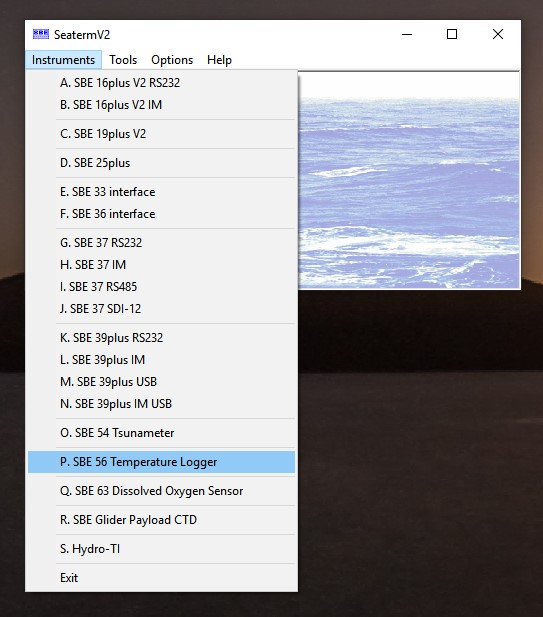
\includegraphics{images/SBE56_program_step_1.jpg}
\item
  Open the housing with the custom endcap remover and connect the SBE 56 to your PC via a USB mini cable.
  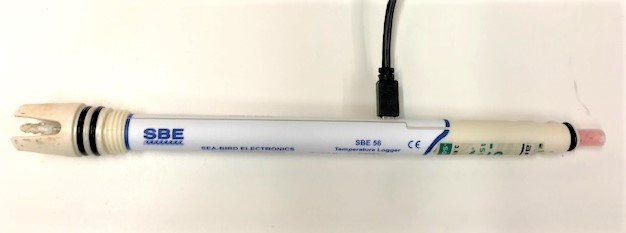
\includegraphics{images/SBE56_connect.jpg}
\item
  When a successful connection is made, you will notice a ``Device Identified'' notification in the bottom left of the screen and you will see the serial number of the unit you have connected to in the upper left of the application window and in the current configuration window.
  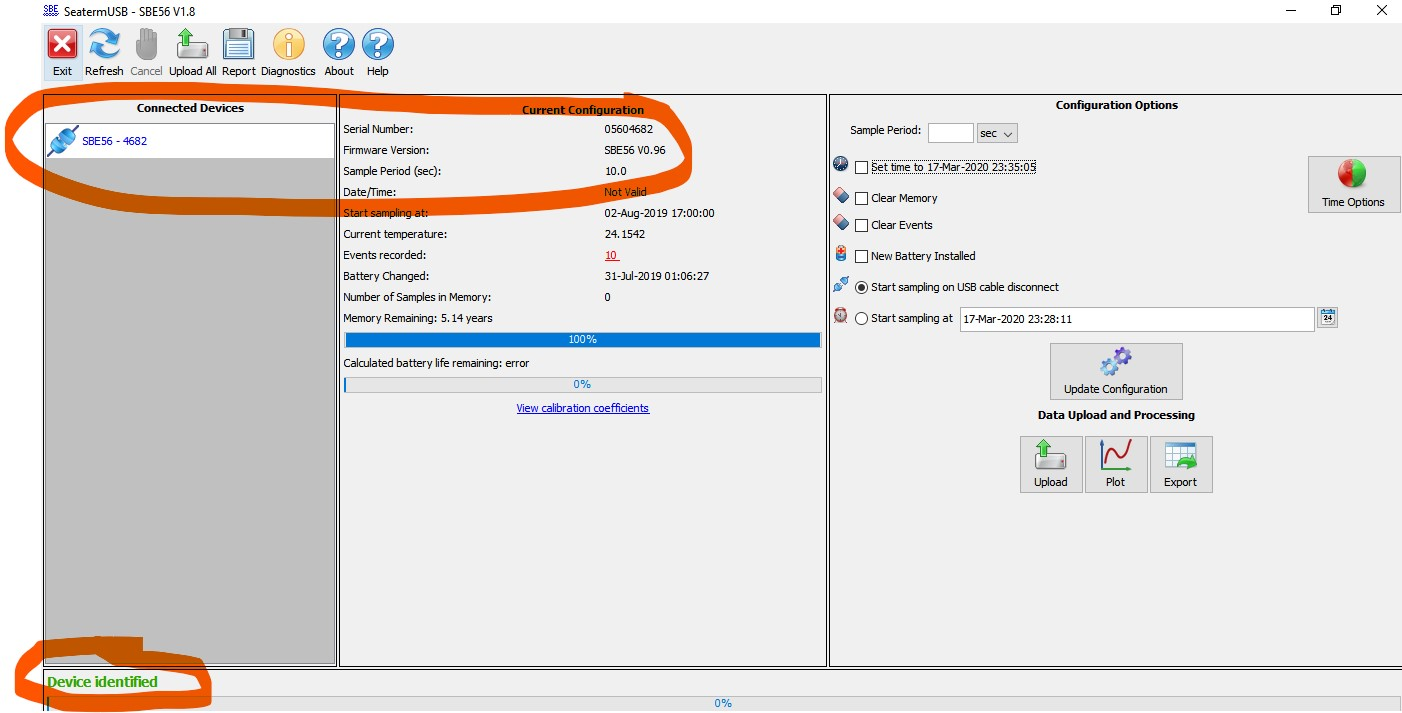
\includegraphics{images/SBE56_program_step_2.jpg}
\item
  Edit the configuration options as follows
\item
  sample period = 5 minutes (300 seconds)
\item
  set time to UTC by clicking the ``time options'' button on the right and select ``GreenWich Mean Time.''
  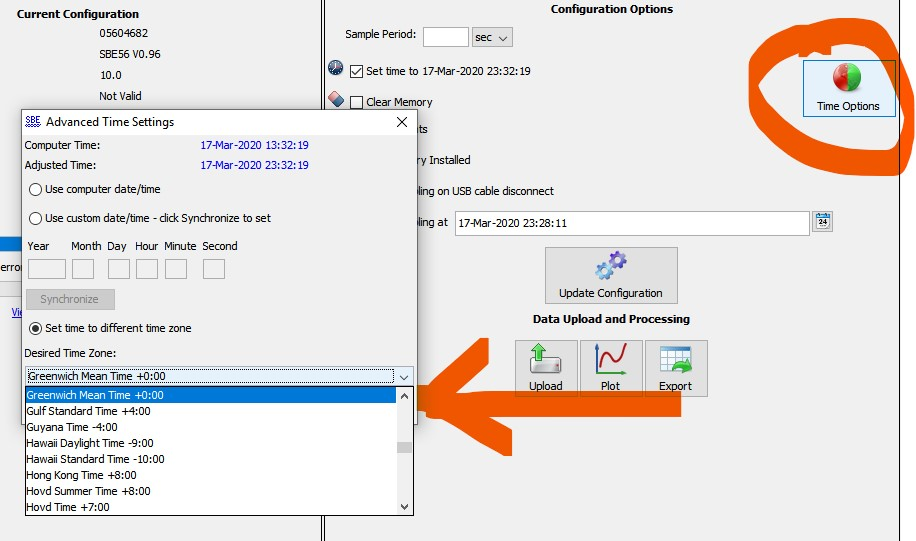
\includegraphics{images/SBE56_program_step_3.jpg}
\item
  check the box for clear memory
\item
  check the boxy for clear events
\item
  check the box for new battery installed (if it is relatively new, which if it is just back from refurbishment, it should be)
\item
  set the date and time for the unit to begin sampling for a time is prior to the day it will be deployed
\item
  When you are done editing the configuration of the SBE56, click the ``Update Configuration'' button and confirm the changes you want to make when the pop-up window asks you to do so. When you have finished, you should see the notification in the bottom left that says, ``finished configuring device - success.'' At this point double check that the ``current configuration'' window on the left shows the parameters that you intended to program the instrument with.
  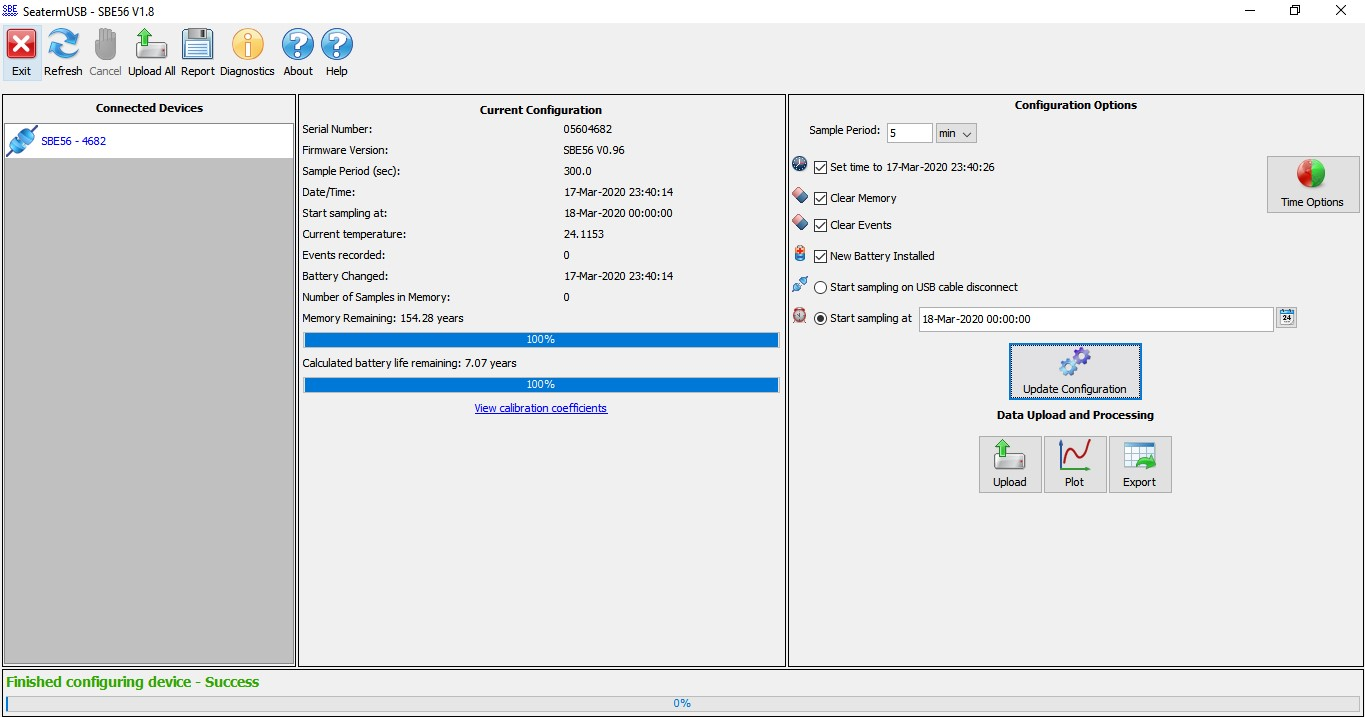
\includegraphics{images/SBE56_program_step_4.jpg}
\item
  At this point, you can disconnect the SBE56, install a new dessicant in its endcap, examine its o-rings for any hairs and re-seal the housing. It is now ready for taping and installation in the deployment bracket.
\end{enumerate}

\textbf{Downloading Data from the SBE56}

\begin{enumerate}
\def\labelenumi{\arabic{enumi}.}
\tightlist
\item
  Connect to the instrument
\end{enumerate}

\textbf{Processing SBE56 Data Files}

see \protect\hyperlink{data_processing}{Data Processing with the OCC Package}

\hypertarget{ctd}{%
\chapter{CTD}\label{ctd}}

\hypertarget{rbr-ctd-in-profiling-mode}{%
\section{RBR CTD in Profiling Mode}\label{rbr-ctd-in-profiling-mode}}

\hypertarget{sbe19-in-profiling-mode}{%
\section{SBE19 in Profiling Mode}\label{sbe19-in-profiling-mode}}

While the SBE 19 is the oldest CTD in the OCC team inventory, it is used as a dedicated shipboard CTD on occaision

\begin{itemize}
\tightlist
\item
  Input commands in upper or lower case letters and register commands by pressing the Enter key.
\item
  If the system does not return an S\textgreater{} prompt after executing a command, press the Enter key to get the S\textgreater{} prompt.
\item
  The SEACAT sends `\#' if an invalid command is entered.
\item
  If a new command is not received within 3 minutes after the completion of a command, the SEACAT returns to the quiescent state and the command/data echo area indicates time out. You must reconnect to the instrument before sending any commands.
\item
  For RS-232 communication: If the instrument is transmitting data and you want to stop it, type \^{}C or press the Esc key or Stop on the Toolbar. Press the Enter key to get the S\textgreater{} prompt.
\item
  Commands marked with * (* is not part of the command) alter the SEACAT's memory and require verification before executing, to prevent accidental modifications.
  After the command entry, SEATERM responds:
  `message' Y/N Type Y and press the Enter key.
  SEATERM then responds:
  are you sure \^{}Y/N Hold down the Ctrl key and type Y (any other response aborts command).
\item
  Braces {[} {]} indicate optional parameters of the command. Items enclosed in braces need not be entered.
\end{itemize}

Find a list of commands for the SBE19 \href{https://docs.google.com/document/d/1WkYxlEDpUm_A1JY6Fx7Kq8Fi2c_drbbzcXDoJRtYLZk/edit}{HERE}

\textbf{example status output of an SBE19 ready to profile after typing ``ds'' and hitting enter}

SEACAT PROFILER V3.1c SN 3029 06/05/18 20:08:52.998
strain gauge pressure sensor: S/N = 2657401406, range = 1000 psia, tc = 194

clk = 32767.852 iop = 148 vmain = 12.2 vlith = 5.1

mode = PROFILE ncasts = 0

sample rate = 1 scan every 0.5 seconds

minimum raw conductivity frequency for pump turn on = 3257 hertz

pump delay = 40 seconds

samples = 0 free = 174128 lwait = 0 msec

SW1 = C8 battery cutoff = 7.3 volts

number of voltages sampled = 0

logdata = NO

S\textgreater ST

date (MMDDYY) = 060518

time (HHMMSS) = 200930

\hypertarget{sbe19plus-in-profiling-mode}{%
\section{SBE19Plus in Profiling Mode}\label{sbe19plus-in-profiling-mode}}

\begin{enumerate}
\def\labelenumi{\arabic{enumi}.}
\tightlist
\item
  Remove the dummy plug from the SBE 19plus' Data I/O 4 pin connector and install the Sea-Bird I/O cable connector, aligning the raised bump on the side of the connector with the large pin (pin 1 - ground) on the SBE 19plus. Plug the serial connector into a serial to usb (Keyspan) converter and plug the USB cable into the computer.
\item
  Open SeaTerm.exe. The display shows the main screen.
\item
  Click Connect on the Toolbar to begin communications with the SBE 19plus. A ``S\textgreater{}'' should be shown on the display if the connection is successful. If it does not show:
  +Click Connect again.
  +Check cabling between the computer and the SBE 19plus.
  +Verify the correct instrument was selected and the COM settings were entered correctly in the Configure menu.
\item
  Display SBE 19plus status information by clicking Status on the Toolbar. The display looks like this:

  \begin{itemize}
  \tightlist
  \item
    SeacatPlus V 1.3 SERIAL NO. 4289 16 July 2005 14:02:13
  \item
    vbatt = 9.6, vlith = 0.0, ioper = 61.2 ma, ipump = 25.5 ma, iext01 = 76.2 ma,
  \item
    status = not logging
  \item
    number of scans to average = 1
  \item
    samples = 5000, free = 376300, casts = 1
  \item
    mode = profile, minimum cond freq = 3000, pump delay = 60 sec
  \item
    autorun = no, ignore magnetic switch = no
  \item
    battery type = ALKALINE, battery cutoff = 7.5 volts
  \item
    pressure sensor = strain gauge, range = 1000.0
  \item
    SBE 38 = no, Gas Tension Device = no
  \item
    Ext Volt 0 = yes, Ext Volt 1 = no, Ext Volt 2 = no, Ext Volt 3 = no
  \item
    echo commands = yes
  \item
    output format = converted decimal
  \item
    output salinity = no, output sound velocity = no
  \end{itemize}
\end{enumerate}

\begin{itemize}
\tightlist
\item
  Make sure in the above information it does not say BATTERY LOW. Batteries should be replaced prior to each cruise; however, it is always good to double check. Ensure UTC time is set correctly. The correct time can be taken from the ship clock or a properly calibrated GPS unit.
\end{itemize}

\begin{enumerate}
\def\labelenumi{\arabic{enumi}.}
\setcounter{enumi}{4}
\tightlist
\item
  When you have confirmed that all data has been obtained from the instrument and you are ready to clear its memmory, send the SAMPLENUMBER=0 or INITLOGGING (e.g.~S\textgreater samplenumber = 0 or S\textgreater initlogging) command to remove unnecessary data files. If one of these commands is not sent, new data will be stored after the last recorded sample, preventing use of the entire memory capacity and make file management more difficult during the next upload.
\item
  Disconnect the Sea-Bird I/O cable connector and screw on the dummy plug. The CTD can be properly stowed until redeployment.
\end{enumerate}

\hypertarget{sbe19plus-in-moored-mode-mode}{%
\section{SBE19Plus in Moored Mode Mode}\label{sbe19plus-in-moored-mode-mode}}

\begin{enumerate}
\def\labelenumi{\arabic{enumi}.}
\tightlist
\item
  Connect instrument and check status: Status \textgreater{} Display status and configuration parameters
\item
  Set date and time under General Setup \textgreater{} Set Date and Time. Date and time are in mmddyyyyhhmmss format (i.e.~6/12/2018 06:15:00 is 06122018061500).
\item
  Clear all past data General Setup \textgreater{} Initialize Logging.
\item
  Set CTD to moored mode under Moored Mode Setup \textgreater{} Set sampling Mode to Moored. Execute command twice to switch to moored mode.
\item
  Set sample interval under Moored Mode Setup \textgreater{} Set Interval (sec) between Samples. For a short deployment (2-4 days), use a sample interval of 10 seconds. For a longer deployment (\textgreater{} 1 week), use a sample interval of 1 min or 5 min.
\item
  Set number of measurements to average under Moored Mode Setup \textgreater{} Set number of measurements to average. Set to 4.
\item
  Set pump mode under Moored Mode Setup \textgreater{} Set Pump Mode to ``pump for 0.5 sec before sampling''.
\item
  Set start date and time under Logging \textgreater{} Set delayed start date and time.
\item
  Start logging under Logging \textgreater{} Start logging when specified by StartDateTime.
  {]}
\end{enumerate}

\hypertarget{downloading-the-sbe19plus}{%
\section{Downloading the SBE19Plus}\label{downloading-the-sbe19plus}}

\begin{enumerate}
\def\labelenumi{\arabic{enumi}.}
\tightlist
\item
  Connect to the 19P with the interface cable.\\
\item
  Open SeaTerm.exe. From the main screen, select the Configure menu. From this menu, select SBE 19plus. Click on the Upload Settings tab. Make sure the Upload Baud Rate reads 9600. In the same menu, click All separated by cast. This allows a separate file to be written for each cast.
\item
  Click Connect on the Toolbar to begin communications with the SBE 19plus. You should see ``S\textgreater{}'' when it connects.
  If the system does not respond as shown above:
\end{enumerate}

\begin{itemize}
\tightlist
\item
  Click Connect again.
\item
  Check cabling between the computer and the SBE 19plus.
\item
  Verify the correct instrument was selected and the COM settings were entered correctly in the Configure menu.
\end{itemize}

\begin{enumerate}
\def\labelenumi{\arabic{enumi}.}
\setcounter{enumi}{4}
\tightlist
\item
  Click the Upload button on the Toolbar to upload stored data
\end{enumerate}

\begin{itemize}
\tightlist
\item
  In the Open dialog box, save the file to the designated location as specified \href{https://drive.google.com/drive/folders/1WcZclgRCLHNOXykYigSZviiwFEH02lKx}{in this Google Drive document}
\end{itemize}

\hypertarget{seafet-ph-sensor}{%
\chapter{SeaFet pH Sensor}\label{seafet-ph-sensor}}

The OCC team uses the SeaBird SeaFet pH sensor as part of the \protect\hyperlink{dielsuite}{Diel Suite} to capture pH information around the clock over a typical deployment interval of 1 to 2 days.

\hypertarget{conditioning-the-seafet-in-seawater-at-least-24-hours-prior-to-deployment}{%
\section{Conditioning the SeaFet in seawater at least 24 hours prior to deployment}\label{conditioning-the-seafet-in-seawater-at-least-24-hours-prior-to-deployment}}

At least 24 hours prior to deployment, the SeaFet must be activated in polled mode (aka low power, aka sleep mode) in a large volume of solution with a similar pH to the pH of the waters in which the unit will be deployed in order to produce accurate data immediately upon deployment. We call this ``conditioning time''. Conditioning in the wetcap with artificial seawater will not work because ionic exchange will quickly change the pH of the small volume of water in the wetcap, thus not actually conditioning the instrument.

\#\#How to Set the SeaFet to polled mode**

\begin{enumerate}
\def\labelenumi{\arabic{enumi}.}
\tightlist
\item
  If needed, install new batteries in the SeaFet (12 Ds)
\item
  Remove dummy plug from endcap of SeaFet and connect SeaFet to computer with USB cable
\item
  Open SeaFetCom software
\item
  Swipe magnet over magnetic switch to ``activate'' batteries (indicator light by magnetic switch will blink green)
\item
  Press ``connect''
\item
  Open settings and confirm operational mode is ``polled mode''
\item
  Click ``upload'' to make sure
\item
  Click ``disconnect''
\end{enumerate}

\hypertarget{programming-the-seafet-for-deployment-after-it-has-already-been-warming-up-in-polled-aka-low-power-sleep-mode-for-at-least-24hrs}{%
\section{Programming the SeaFet for Deployment (After it has already been warming up in polled, aka low power sleep mode for at least 24hrs)}\label{programming-the-seafet-for-deployment-after-it-has-already-been-warming-up-in-polled-aka-low-power-sleep-mode-for-at-least-24hrs}}

\textbf{In the dry lab prior to deployment}

At least \textbf{24 hours} prior to deployment: install and activate internal batteries. To activate internal batteries, swipe the magnet to the target until the indicator LED starts flashing green (this may take a few attempts). Alternatively, connect the instrument to the computer and place in \textbf{periodic mode} following instructions below.

\begin{enumerate}
\def\labelenumi{\arabic{enumi}.}
\item
  Remove the dummy plug and connect data logger cable.
\item
  Open SeaFETCom and select ``Connect to SeaFET'' to begin communications with instrument.
\item
  Sync instrument clock with computer clock: Sensor -\&gt; Set Clock, ``Sync Time'' . Instrument time should be in UTC.
\item
  To access SeaFET deployment settings, select the ``SeaFET Settings'' button in the dashboard window or Sensor -\&gt; ``SeaFET Settings''. Use the following settings:
\end{enumerate}

\textbf{General}

\textbf{Operational Mode:} Periodic

\textbf{Sample Interval} : 1 min

\textbf{Offset} : 0 sec

\textbf{Number of samples in average:} 30

\textbf{Number of frames in burst:} 1

\textbf{Enable Sampling Window} : If using, check box and set appropriate start and end dates

*We haven't been able to make this work well, so don't use sampling interval for now*

\textbf{Internal Device Logging}

** Logging level:** INFO

\textbf{Maximum log file size:} 9999 KB

\textbf{Telemetry}

\textbf{Serial Baud Rate:} 57600

\textbf{Transmitted Frame Format:} FULL\_ASCII

\textbf{Instrument Logging Frame Format:} FULL\_ASCII

\textbf{Log File Creation Method} : By file size

\textbf{Maximum Size:} 9999 KB

\textbf{Uncheck}``legacy format''

\textbf{Processing}

\textbf{Salinity} : 35 psu

\textbf{External Pump} - no external pump in use

\textbf{CTD} -- no CTD in use

Note: For RAMP deployments, the SeaFET will be deployed in \textbf{periodic mode} , in which it will sample at a specified interval and burst size and go to sleep in between measurements. The instrument can be put in \textbf{polled mode,} in which it remains in a low power sleep state until woken by an external command, for long-term storage or shipping. \textbf{Continuous mode} should only be used when the instrument is powered by an external power source.

\textbf{Activiate the instrument prior to getting on the small boat}

\begin{enumerate}
\def\labelenumi{\arabic{enumi}.}
\tightlist
\item
  Start deployment by selecting the ``Start'' button in the SeaFETCom dashboard or Sensor -\&gt; ``Start''.
\item
  Disconnect from SeaFET, remove data logger cable, and replace dummy plug.
\end{enumerate}

\textbf{On the small boat}

\begin{enumerate}
\def\labelenumi{\arabic{enumi}.}
\tightlist
\item
  Immediately prior to deployment, remove wet cap. Remove two stainless steel plugs and store securely. Invert the instrument to pour the storage solution from the wet cap into a sink. Using a 5/32" hex driver or Allen key, remove the three 10-32 x 5/8" socket head cap screws from the wet cap. Remove the wet cap.
\item
  Install foul guard. Place instrument on a flat surface with the sensor end cap up. Place the electrode foul guard over the electrode. Insert the three 10-32 x 5/8" socket head cap screws removed from wet cap and tighten completely. Sensor end cap should not be exposed to air for more than a few seconds, so submerge in water if not immediately deploying underwater.
\end{enumerate}

\textbf{Retrieving the SeaFet}

\begin{enumerate}
\def\labelenumi{\arabic{enumi}.}
\tightlist
\item
  Upon recovery of the instrument, stick the wetcap end into a bucket of seawater for return to the ship or remove foul guard and replace wet cap. Ensure wet cap is filled with sterilized, artificial seawater or filtered seawater. Keep the sensor end wet at all times (it can be without water no more than an hour).
\end{enumerate}

\hypertarget{downloading-data-from-the-seafet}{%
\section{Downloading Data from the SeaFet**}\label{downloading-data-from-the-seafet}}

\begin{enumerate}
\def\labelenumi{\arabic{enumi}.}
\setcounter{enumi}{1}
\item
  Remove dummy plug, attach data logger cable, and connect to SeaFETCOM software.
\item
  Select ``Transfer Files'' from the SeaFETCom Dashboard.
\item
  In the ``Local Filesystem'' pane, press ``Browse'' to select the local folder on the computer that will receive downloaded files.
\item
  In the ``Instrument Filesystem'' pane, select the files to be downloaded from the SeaFET and press the ``\&lt;-'' button to transfer selected files.
\end{enumerate}

\begin{itemize}
\tightlist
\item
  A Seafet deployment creates 2 file types: a log file that contains metadata about the deployment and the data file (may be more than one data file)
\end{itemize}

\begin{enumerate}
\def\labelenumi{\arabic{enumi}.}
\setcounter{enumi}{5}
\tightlist
\item
  If the instrument will be used in the near future, place in \textbf{polled mode} following deployment steps above. This low-power stand-by mode will maintain a continuous current flow to the sensing element and eliminate the need for a 24-hour warmup. If the instrument will not be used in the near future, deactivate internal batteries by swiping the magnet over the target until the LED flashes red.
\end{enumerate}

\hypertarget{properly-store-the-seafet}{%
\section{Properly Store the SeaFet}\label{properly-store-the-seafet}}

It is crucial to store the SeaFET sensors with clean seawater in the wet cap. If seawater is not available, artificial seawater will suffice. The internal KCl reference gel in the DuraFET will become dry if left out of water, resulting in calibration drift and potentially causing irreversible damage. \textbf{Do not store} the SeaFET with freshwater in the wet cap, as this will change the chemistry of the external reference electrode.

If storing or shipping the SeaFET, disconnect the batteries in SeaFETCOM:

\begin{itemize}
\tightlist
\item
  Connect the SeaFET to SeaFETCom
\item
  Navigate to Sensor \&gt; Advanced \&gt; Disconnect for Storage.
\end{itemize}

This will disconnect the isolated battery pack from the external reference sensor to retain battery life.

\hypertarget{email-exchanges-about-seafet-for-reference}{%
\section{Email Exchanges about Seafet for reference}\label{email-exchanges-about-seafet-for-reference}}

\textbf{Notes on SeaFet soaking and response time}

February 12, 2018 Hi Noah,

\textbf{Yes indeed, if you are concerned about the time it takes to stabilize, you could combat this by immersing in some seawater that is close to the sites parameters ahead of time.}

\textbf{Know however, that having the SeaFET running in the small volume of water within the wetcap, it will quickly become altered from normal regarding the small volume and ionic exchange.}

\textbf{(This might be the reason why you mentioned the pH value of 6 in the wetcap currently.)}

\textbf{Ideally one would want to have a larger water} volume however this might require some creativity to accomplish !

Proposed settings look fine !

Regarding a specific start time:

Within SeaFETCom - SeaFET Settings - In the SeaFET General Settings Tab you can select the desired Start date, but I not Believe you can specify the time of day.

But looking into the firmware commands it appears the SeaFET can be programmed with a start time as well.

At the SeaFET's command prompt, enter the following commands as an example: ``set --samplwin true'' and then "set --samstart yyyy/mm/dd.hh:mm:ss

Note these commands can be sent using the ``Command Terminal'' found under Sensor Menu - Advanced in SeaFETCom, or through TeraTerm direct serial connection.

I believe programming in periodic mode, with a delayed start up time would achieve the same effect.

Please let me know if you have any questions or comments.

Kind Regards,
Darrell

\begin{longtable}[]{@{}l@{}}
\toprule
February 9, 2018 Email from Darrel at Seabird Tech Support:\tabularnewline
\midrule
\endhead
\bottomrule
\end{longtable}

\begin{longtable}[]{@{}l@{}}
\toprule
\endhead
\bottomrule
\end{longtable}

Hello Noah,

Thank You for your email !

\begin{itemize}
\tightlist
\item
  Is 24hrs adequate for the instrument to ``warm up'' in polled mode (I believe you've called this ``conditioning mode'' before) prior to deployment or are multiple days necessary?
\end{itemize}

\textbf{The time of }** SeaFET ****'s sensors adjusting to the in-situ environment can vary. Really it depends on how different the water is from the storage solution.
When we perform calibration it can take anywhere for a day, to several days - but we are looking for high level of stability.
When deploying the **** SeaFET **** the pH values may take a couple of days for the readings to stabilize to the environment.**

\begin{itemize}
\tightlist
\item
  How long can the sensor be exposed to air before damage to the sensor occurs? (We are wondering about best practices for taking the instrument from the small boat into the water. For instance, the wetcap remains on the instrument until we get to the dive site. We get to the dive site and prepare our SCUB gear, then remove the wetcap and affix the protective copper endcap over the sensor - at this point, 1 to several minutes my pass before it is actually submerged in the ocean when we roll in the water.)
\end{itemize}

\textbf{I do not see a problem here. For damage to occur to the ISFET it will have to become dry. I would say best practice would be no more than 1 hour. But a couple of hours will not cause damage, just likely additional time to reach stability in the new environment. The external reference can become dry without damage - but some further conditioning time would be expected.}

\begin{itemize}
\tightlist
\item
  Is setting the instrument to periodic mode with a future sample start date considered a low power mode, comparable to ``polled mode''
\end{itemize}

Yes I believe this would achieve the same, however you would need to ensure to switch to polled mode if this is method use during deployment.
If you have an external controller, polled is likely the better option for use. If you were using periodic mode and an external device collecting the SeaFET's data - this would rely on the two systems have no change in the their clocks. Polled mode would be better as the external controller would be able to collect data whenever it chooses.

I hope this helps !

Please let me know if you have any questions or comments.

Kind Regards,
Darrell

\textbf{Greg Ikeda} Thu, Oct 1, 2015 at 10:44 AM

Hi Noah,

You've brought up some good questions about the SeaFET- I went ahead and consulted our engineer responsible for this instrument to obtain some more concrete answers.

SeaFET soak time:

Craig is correct- the SeaFET requires a ``conditioning time'' that allows the sensors to stabilize before achieving full accuracy. I've attached a paper that explores the best practices for obtaining quality data from the SeaFET. Please reference this document for quality control procedures. From this paper:

Upon first contact with seawater, pH sensor voltages relative to both reference electrodes exhibit an asymptotic
drift. This conditioning period arises from several sources:

\begin{enumerate}
\def\labelenumi{\arabic{enumi})}
\item
  Achieving a stable flow of ions across the liquid junction of the internal reference electrode (nominally hours),
\item
  replacement of Cl -- with Br ? in the solid solution of AgCl of the Cl-ISE (nominally days),
\item
  an ISFET conditioning component, related to the initial power-up of the chip, the exact basis of which is not fully understood (nominally 1 day), and
\item
  a pressure effect on the ISFET and internal reference electrode through changes in the liquid junction potential that may become important if the sensor is deployed more than 20 m below the surface (nominally 1 h).
\end{enumerate}

Factors 1--3 can be addressed by operating the pH sensor continuously in seawater (never powering off the ISFET) for one week prior to deployment and taking care to keep the sensor wetted in natural seawater during transport.

SeaFET response time:

It very much depends on the system at hand. After initial conditioning (as described above):

\begin{enumerate}
\def\labelenumi{\alph{enumi})}
\item
  With continuous water flow, either naturally occurring or forced, the response is practically instantaneous.
\item
  If the sensor has to re-condition to a new volume of water for every measurement, it could take up to 30sec to converge to the right number. For the SeapHox we added a configuration parameter to delay the measurement for this reason.
\end{enumerate}

These reasons certainly make the SeaFET a poor match for use on a moving platform. I hope this clarifies your questions about the SeaFET. Please review the attached paper and let us know if you have additional questions.

Regards,

Greg

Greg Ikeda
Technical Support
Sea-Bird Electronics
13431 NE 20th Street
Bellevue, Washington 98005
Telephone: \href{nulltel:\%28\%2B1\%29\%20425-643-9866}{(+1) 425-643-9866}
Fax: \href{nulltel:\%28\%2B1\%29\%20425-643-9954}{(+1) 425-643-9954}
E-mail: \href{nullmailto:gikeda@seabird.com}{gikeda@seabird.com}
Web: \href{http://www.seabird.com/}{http://www.seabird.com}

\hypertarget{puc}{%
\chapter{PUC - Portable Underwater Collector}\label{puc}}

Part of the \protect\hyperlink{dielsuite}{diel suite}, the Programmable Underwater Collector (PUC) is a moored instrument used to collect water samples autonomously at pre-determined times. The OCC team uses the PUC to analyze the diel carbonate cycle at study sites.

\hypertarget{general-notes}{%
\section{General Notes}\label{general-notes}}

\begin{itemize}
\item
  Decide on sampling interval for deployment period
\item
  There are 3 versions of PUCS with different O rings
\item
  See PUC fill time table below to program each PUC with a specific pump time to achieve the desired 800 mL in each tedlar sample bag
\item
  Batteries: use one change of 12 AA alkaline batteries for two deployments
\item
  Red ON/OFF switch mounted on motherboard

  \begin{itemize}
  \tightlist
  \item
    turn to ON when PUC in to be used.
  \item
    when ON, access Basic stamp Editor using magnet+PUC comm cable.
  \item
    when ON, flush tubing prior to deployment using magnet.
  \item
    turn to OFF when PUC in storage. No need to remove AA batteries.
  \end{itemize}
\end{itemize}

\hypertarget{preparation-the-day-before-deployment}{%
\section{Preparation the Day Before Deployment}\label{preparation-the-day-before-deployment}}

Mount PUCs to crates with cable tieas, 3 PUCs per crate. Print out the \href{https://drive.google.com/drive/folders/1X6fAG4OIDs66Ji5xzYsX8JySqhkSs5k-}{PUC deployment underwater checklist at this Google Drive link}

\textbf{Preparing 1L tedlar sample bags with mercuric chloride}

\begin{enumerate}
\def\labelenumi{\arabic{enumi}.}
\tightlist
\item
  Label the bags with a large chisel tip sharpie with the hour they will sample in 24hr time format
\item
  Open bag valve 1 full turn
\item
  Evac air out of bag with plastic syringe
\item
  Close bag valve while syringe is attached and vacuum is apparent
\item
  Load up glass syringe with 200 ul HGCL2, draw it carefully, tap to remove air
\item
  Insert syringe needle through septum and inject HGCL2
\end{enumerate}

\hypertarget{programming-pucs-with-firmware-version-2018-jan-7}{%
\subsection{Programming PUCS with firmware version 2018-JAN-7}\label{programming-pucs-with-firmware-version-2018-jan-7}}

\textbf{Note: This should take place the night before the planned deployment}

\begin{enumerate}
\def\labelenumi{\arabic{enumi}.}
\item
  If necessary, install 12 new AA alkaline batteries into the PUC (one set of batteries is used for 2 deployments)
\item
  Open the PUC carefully with the PUC opener tool
\item
  Connect the PUC to your PC with the RS232 (serial) cable and a Keyspan USB to serial adapter. NOTE: It may be necessary to plug the USB cable into a ``high-power'' USB port on your PC. If using the instrument computer PICSC26, this is the USB port that has a lighting bolt symbol over it
\item
  Turn on the red power on/off switch on the PUC motherboard
\end{enumerate}

\textbf{Open the Basic Stamp Editor program}

\begin{enumerate}
\def\labelenumi{\arabic{enumi}.}
\item
  Select Run then Debug then New to open a programming terminal
\item
  If the PUC does not connect, try selecting a different com port
\item
  Individual PUC d1eployment status is displayed
\item
  Check the date, time, pump time and programmed time (the PUC pump will run for 10 seconds while you review this information, at the end of the 10 sec period, you will have 30 sec waiting period to input commands into the terminal before the pump runs again and re-displays current settings. If you do not enter commands within the 30s window, the program will time out and you must swipe the magnet over the magnetic switch (red dot on endcap) to start a new 30s programming window)
\item
  Set parameters for the deployment keying and pressing enter for numbers 1-4 that correspond to the following:

  \begin{itemize}
  \tightlist
  \item
    set Date/Time: MM/DD/YY, HH/MM
  \item
    Display Date/Time: to display the date time programmer has entered.
  \item
    set sample Date and Time: MM/DD/YY, HH/MM (we set PUCs to UTC time, use \href{https://drive.google.com/drive/folders/1aprNsz_a0cfscmCBz0DjbCuvCFerOfaw}{the PUC deployment planning and data sheet at this Google Drive link} to determine the proper UTC time according to the local solar time), and Pump Time (the amount of time in minutes that the pump runs to collect the water sample.
  \end{itemize}
\item
  If the PUC time reads more than 60 seconds, run the script in the basic stamp editor to correct this: PUC Clock Fix\_DS1302\_Demo.bs2 found \textbf{where is this file, when found we need to put it in the PUC google drive folder?}
\end{enumerate}

\begin{itemize}
\tightlist
\item
  Then open the latest firmware from basic stamp from the \href{https://drive.google.com/drive/folders/1X6fAG4OIDs66Ji5xzYsX8JySqhkSs5k-}{PUC Google Drive Folder}: PUC firmware upgrade 07Jan18.bs2
\item
  note: You may need to change the comp port number in the top line of code
\end{itemize}

\begin{enumerate}
\def\labelenumi{\arabic{enumi}.}
\setcounter{enumi}{6}
\item
  Start Sample Program, results in the PUC displaying ``Entering sample Mode'' + Sample Time + Pump Time + current Date/Time
\item
  NOTE: all PUCs do not pump at the same rate. We aim to have 800mL of water in each 1L bag. The time it takes for a pump to fill a bag to 800mL varies from 27-36 minutes; see the chart below of PUC times in the next and program each PUC accordingly.
\item
  The final program step is ALWAYS press \#4 to get ``Entering sampling Mode'' prompt. Confirm sample date/time and pump time.
\item
  Pre-fill a Diurnal Suite Datasheet Spreadsheet with relevant information for the deployment
\item
  After programming is complete and all parameters are verified, seal the PUC
\end{enumerate}

\begin{itemize}
\tightlist
\item
  clean/lubricate o-ring.
\item
  Install one large or several small desiccants inside the PUC, ideally rubber banded to the motherboard or battery packs somehow
\item
  hand tighten PUC cap to PUC body using PUC opener tool
\end{itemize}

\hypertarget{puc-rates-and-fill-times-as-of-june-2018}{%
\section{PUC Rates and Fill Times (As of June 2018)}\label{puc-rates-and-fill-times-as-of-june-2018}}

\begin{longtable}[]{@{}lll@{}}
\toprule
\textbf{PUC SN} & \textbf{Time to 800mL (minutes)} & \textbf{March 2018 Tested Rate (mL/min)}\tabularnewline
\midrule
\endhead
1 & 39 & 20.6\tabularnewline
2 & 30 & 26.4\tabularnewline
3 & 31 & 25.5\tabularnewline
4 & 32 & 24.7\tabularnewline
5 & 33 & 23.9\tabularnewline
6 & 39 & 20.6\tabularnewline
7 & 32 & 25.2\tabularnewline
8 & 29 & 27.4\tabularnewline
9 & 37 & 21.8\tabularnewline
\bottomrule
\end{longtable}

\textbf{Don't Overfill Those PUC Bags!}

\includegraphics[width=8.89in]{images/PUC_bag_pop}

\hypertarget{puc-deployment}{%
\section{PUC Deployment}\label{puc-deployment}}

\begin{enumerate}
\def\labelenumi{\arabic{enumi}.}
\tightlist
\item
  Ensure PUCs are fastened securely to the milk crate (maximum 4 PUCs per crate)
\item
  With tubing connected to ``water out'' valve tip but NOT YET to the tedlar bag, swipe the magnetic switch (red dot) on PUC endcap to run the pump once to pump ambient seawater through the tubing.
\item
  Connect the other end of the tubing to the ``water in'' valve tip of the tedlar bag
\item
  Open tedlar bags by turning valve one full turn
\end{enumerate}

\hypertarget{puc-recovery}{%
\section{PUC Recovery}\label{puc-recovery}}

Print out the \href{https://drive.google.com/drive/folders/1X6fAG4OIDs66Ji5xzYsX8JySqhkSs5k-}{PUC retreival underwater checklist at this Google Drive link}

\begin{enumerate}
\def\labelenumi{\arabic{enumi}.}
\tightlist
\item
  Gather tools needed

  \begin{itemize}
  \tightlist
  \item
    Zip tie snips
  \item
    Goody bag for collecting filled Tedlar bags
  \item
    50lb open bottom lift bag and carabiner to lift milk crates
  \item
    A few extra large (at least 2ft cable ties)
  \end{itemize}
\item
  Close valves on all sample bags
\item
  Remove tubing from sample bag valves
\item
  Use snips Carefully collect tedlar bags and snow in a goody bag dedicated solely to them for safe ascent; be careful when handing them up out of the water to whoever receives them on the small boat
\item
  Secure the two milk crates together with zip ties if not already fastened together for easier lifting
\item
  Affix 50lb lift bag with carabiner to milk crates in a secure fashion and make a safe ascent
\item
  Upon surfacing, instruct whomever is grabbing the tedlar bag samples from you to carefully place them into a CAU bucket filled with water to reduce pressure on the bags
\end{enumerate}

\textbf{Transfer of Samples from Tedlar Bags to Glass Bod Bottles in Wetlab}

\hypertarget{notes-from-chris-langdon-about-pucs}{%
\subsection{Notes from Chris Langdon about PUCs}\label{notes-from-chris-langdon-about-pucs}}

Notes from Chris Langdon:

\begin{itemize}
\tightlist
\item
  9/14/15 email: The new boards have a voltage regulator that can be set to 11.0 volts if only one pump is used and to 13.0 volts if two pumps are used (this gives the motor more torque needed to drive two pumps).
\item
  O-rings you need for the two styles of PUCs. Order from McMaster Carr. The o-rings should easily last a year. I would suggest replacing them annually.
\end{itemize}

Old style cap ---- dash\# 2-153. McM. 9452K174

New style cap---- dash\# 2-236 McM 9452K165

\begin{itemize}
\item
\item
  1/6/2018 email about new firmware: It gives you 30 sec to hit a key about the pump starts running. I also reduced the pump run time to 10 seconds. You can now specify the month, day, hour and minute that the PUC will sample so you can set it up days in advance. You will need the Basic Stamp editor application downloaded from Paralax.
\end{itemize}

\hypertarget{aquadopp-nortek-adcp}{%
\chapter{Aquadopp: Nortek ADCP}\label{aquadopp-nortek-adcp}}

\begin{itemize}
\tightlist
\item
  2MHZ aquadopps have a shorter range (20m I think)
\end{itemize}

\hypertarget{programming-the-aquadopp}{%
\section{Programming the Aquadopp}\label{programming-the-aquadopp}}

\begin{enumerate}
\def\labelenumi{\arabic{enumi}.}
\tightlist
\item
  Connect to the Aqudopp with the interface cable
\item
  Open Nortek software
\item
  From the Communication menu, select the correct com port for the instrument's interface cable (look this up in the device manager)
\item
  Communications -\&gt; connect (if it does not connect, the instrument's batteries may be dead; use the AC power adapter)
\item
  ``Erase Recorder''
\item
  Set clock to UTC time: On-line -\&gt; set clock
\item
  Deploy-\&gt;planning-\&gt; load from file then chose``PUC\_24HR\_1Mhz'' con file
\item
  If you can't find the file, use these settings:
\item
  Frequency: 1 Mhz
\item
  Profile interval: 300 seconds
\item
  Number of cells: 20
\item
  Cell size: 1 m
\item
  Start logging under Deployment \&gt; Start Recorder Deployment. File name and comments should include island code and cruise year.
\item
  Prep instrument for deployment
\item
  Clean O-rings, replace battery (if needed)
  1. When opening the end cap, make sure to unscrew the screws a bit at a time, alternating screws, so that the end cap comes off evenly
\item
  Plug in battery and end cap, add dessicant to battery case, close cap
  1. Make sure battery fabric doesn't get pinched in end cap
  2. Screw on cap a little at a time, alternating screws, to not bend or damage screws/cap
\item
  Note: Nortek recommends a 10V minimum cutoff voltage.
\end{enumerate}

\hypertarget{deploying-the-aquadopp}{%
\section{Deploying the Aquadopp}\label{deploying-the-aquadopp}}

\begin{itemize}
\tightlist
\item
  Orient the aquadopp so that the length of it's body is flat in relation to the surface of the ocean and that the head is also rotationally flat relative to the surface of the ocean
\item
  Upon deployment shoot a bearing on positive X, take a picture of compass upon deployment
\item
  Deploy instrument

  \begin{itemize}
  \tightlist
  \item
    Make sure it is pointing up, relatively flat, and solidly attached to something (NO WIGGLING)
  \item
    The ADCP head should not be closer than 10 instrument diameters to any structure that is taller than the instrument head

    \begin{itemize}
    \tightlist
    \item
      Otherwise the beams will bounce off of the tall object, giving bad readings
    \end{itemize}
  \item
    Take a compass heading on deployment and record it if instrument is recording in xyz coordinates
  \end{itemize}
\end{itemize}

\hypertarget{retrieve-the-aquadopp}{%
\section{Retrieve the Aquadopp}\label{retrieve-the-aquadopp}}

\begin{enumerate}
\def\labelenumi{\arabic{enumi}.}
\tightlist
\item
  Recover instrument
\item
  Download and process data
\item
  Download data using Aquadopp software; Deployment \&gt; Recorder Data Retrieval. Saves as .prf file.
\item
  Process using R package occ `processADCP' function.
\end{enumerate}

\hypertarget{shipboard-operations}{%
\chapter{Shipboard Operations}\label{shipboard-operations}}

Note: since the Hiialakai was decommissioned in 2019, no plans have been made to re-install the PCO2 or TA system on another vessel

\hypertarget{pco2-system}{%
\section{PCO2 System}\label{pco2-system}}

\begin{itemize}
\tightlist
\item
  Perform simple check of system daily (see to-be-developed checklist)
\item
  \href{https://drive.google.com/drive/folders/1p-Evjb3zrw4Kk460knsl4rI4m2Un_jyy}{See detailed documentation in this Google Drive Folder Link}
\end{itemize}

\hypertarget{ta-system}{%
\section{TA System}\label{ta-system}}

Perform simple check of system daily (see to-be-developed checklist)

\begin{itemize}
\tightlist
\item
  \href{https://drive.google.com/drive/folders/1p-Evjb3zrw4Kk460knsl4rI4m2Un_jyy}{See detailed documentation in this Google Drive Folder Link}
\end{itemize}

\hypertarget{tasks}{%
\chapter{Tasks at Sea}\label{tasks}}

\hypertarget{daily-tasks-for-the-team}{%
\section{Daily Tasks for the Team}\label{daily-tasks-for-the-team}}

\href{https://drive.google.com/open?id=1I4Hojo0qjKtUwhRqgc9aLM6_fGtjqZMM}{Find Excel version here via Google Drive}

\textbf{STR}

\begin{itemize}
\tightlist
\item
  Before Ops

  \begin{itemize}
  \tightlist
  \item
    assemble, program and stage needed STRs
  \item
    confirm 10 36'' cable ties for each STR planned
  \item
    write serial numbers of planned STR deployments on tomorrow's data sheet
  \end{itemize}
\item
  After Ops

  \begin{itemize}
  \tightlist
  \item
    download strs
  \item
    enter deployments and retreivals into mooring database
  \item
    import waypoints into mooring database
  \item
    clean STRs, put weights and brackets on fantail or in DD bath
  \end{itemize}
\end{itemize}

\textbf{CAU}

\begin{itemize}
\tightlist
\item
  Before Ops

  \begin{itemize}
  \tightlist
  \item
    Pack supplies for planned CAU site swaps
  \item
    write down deploy CAU SNs on tomorrow's data sheet
  \end{itemize}
\item
  After Ops

  \begin{itemize}
  \tightlist
  \item
    scrape/record CAU SN's, re-bag and freeze with cruise \& site label
  \item
    dispose of old clips and stakes
  \item
    after CTD/H2O data is entered, give data sheets to data manager
  \end{itemize}
\end{itemize}

\textbf{Water Sampling and CTD}

\begin{itemize}
\tightlist
\item
  Before Ops

  \begin{itemize}
  \tightlist
  \item
    DIC bottles and all supplies in each kit
  \item
    Niskin, line, messenger, weight staged for each CTD
  \end{itemize}
\item
  After Ops

  \begin{itemize}
  \tightlist
  \item
    rinse and stage CTDs
  \item
    Swap full bottles for empties, dispose of waste
  \item
    restock all supplies
  \item
    replace and label any worn ziplocs
  \item
    enter CTD and water sample log into CTD/H2O Database (hopefully this is not a necessary step on MARAMP 2020!)
  \end{itemize}
\end{itemize}

\textbf{GPS Units (for OCC and benthic/fish GPS)}

\begin{itemize}
\tightlist
\item
  Drop off GPS units with data manager for waypoiont download
\end{itemize}

\textbf{Cameras}

\begin{itemize}
\tightlist
\item
  Before Ops

  \begin{itemize}
  \tightlist
  \item
    Ensure cameras are set to UTC time
  \item
    Ensure cameras have memory cards
  \item
    charge camera batteries
  \item
    clean camera housings
  \item
    bake desiccants and install them
  \end{itemize}
\item
  After Ops

  \begin{itemize}
  \tightlist
  \item
    download and sort photos
  \item
    download and sort photoquad photos
  \item
    charge cameras or swap charged batts for used batts
  \item
    install new dessicants
  \end{itemize}
\end{itemize}

\textbf{Stage all Gear}

\begin{itemize}
\tightlist
\item
  Action packer packed for day of ops
\item
  Pam float and reel staged
\item
  If deep STR: Marker Float and drop weight
\item
  1 full bag of large cable ties (keep on boat)
\item
  CTDs and lines
\end{itemize}

\textbf{Other}

\begin{itemize}
\tightlist
\item
  gauge tanks
\end{itemize}

\textbf{Team Lead}

\begin{itemize}
\tightlist
\item
  Plan tomorrow's objectives
\item
  Plan and communicate tank needs to team members
\end{itemize}

\hypertarget{where-to-save-data}{%
\section{Where to Save Data}\label{where-to-save-data}}

\href{https://drive.google.com/open?id=16l1OQgGEunLoADh_MEGyIfbQL2w0u6aw}{Checkout this Excel file on Google Drive for details on where to save data}

\hypertarget{data_how_to}{%
\chapter{Data How To}\label{data_how_to}}

\hypertarget{how-to-gain-access-to-the-occ-database}{%
\section{How to Gain Access to the OCC Database}\label{how-to-gain-access-to-the-occ-database}}

As of January 2020, the OCC team is in the process of working with the data management team to migrate all OCC Team data and metadata to an Oracle database. In order to access this database, a new user must submit an \href{https://www.st.nmfs.noaa.gov/jira/login.jsp?permissionViolation=true\&os_destination=\%2Fbrowse\%2FPICITS-181121\%3Ffilter\%3D-2\&page_caps=\&user_role=}{ITS support ticket} to request an Oracle account in addition to requesting an install of SQL Developer. If you'd like to access data via R, you'll also need to request to have ODBC drivers setup.

\hypertarget{how-to-archive-data}{%
\section{How to Archive Data}\label{how-to-archive-data}}

After data is qc'd it mus be archived. As of January 2020, the best place to look for all information and guidance related to archiving data is in a \href{https://drive.google.com/drive/folders/1Oq76hN6eOhhJOevwZiO0nX4Gtf0tiJrp}{google drive folder setup by Annette}.

\hypertarget{how-to-connect-to-the-oracle-database}{%
\section{How to Connect to the Oracle Database}\label{how-to-connect-to-the-oracle-database}}

\href{https://docs.google.com/document/d/19hVuyRj78kB3NHR4xF-mWZeOZCwYMDNSLSwQc08Af7s/edit\#}{Checkout this live SOP on Google Drive for how to get connected to OCC Data in the oracle database}

\hypertarget{how-to-connect-to-the-occ-oracle-databse-via-oracle-sql-developer}{%
\section{How to Connect to the OCC Oracle Databse Via Oracle SQL Developer}\label{how-to-connect-to-the-occ-oracle-databse-via-oracle-sql-developer}}

\begin{enumerate}
\def\labelenumi{\arabic{enumi}.}
\tightlist
\item
  Open Oracle SQL Developer
\item
  On the ``Welcome Page'' tab, under the ``Databases Detected'' tab, find the ``GIS'' database and click it.
  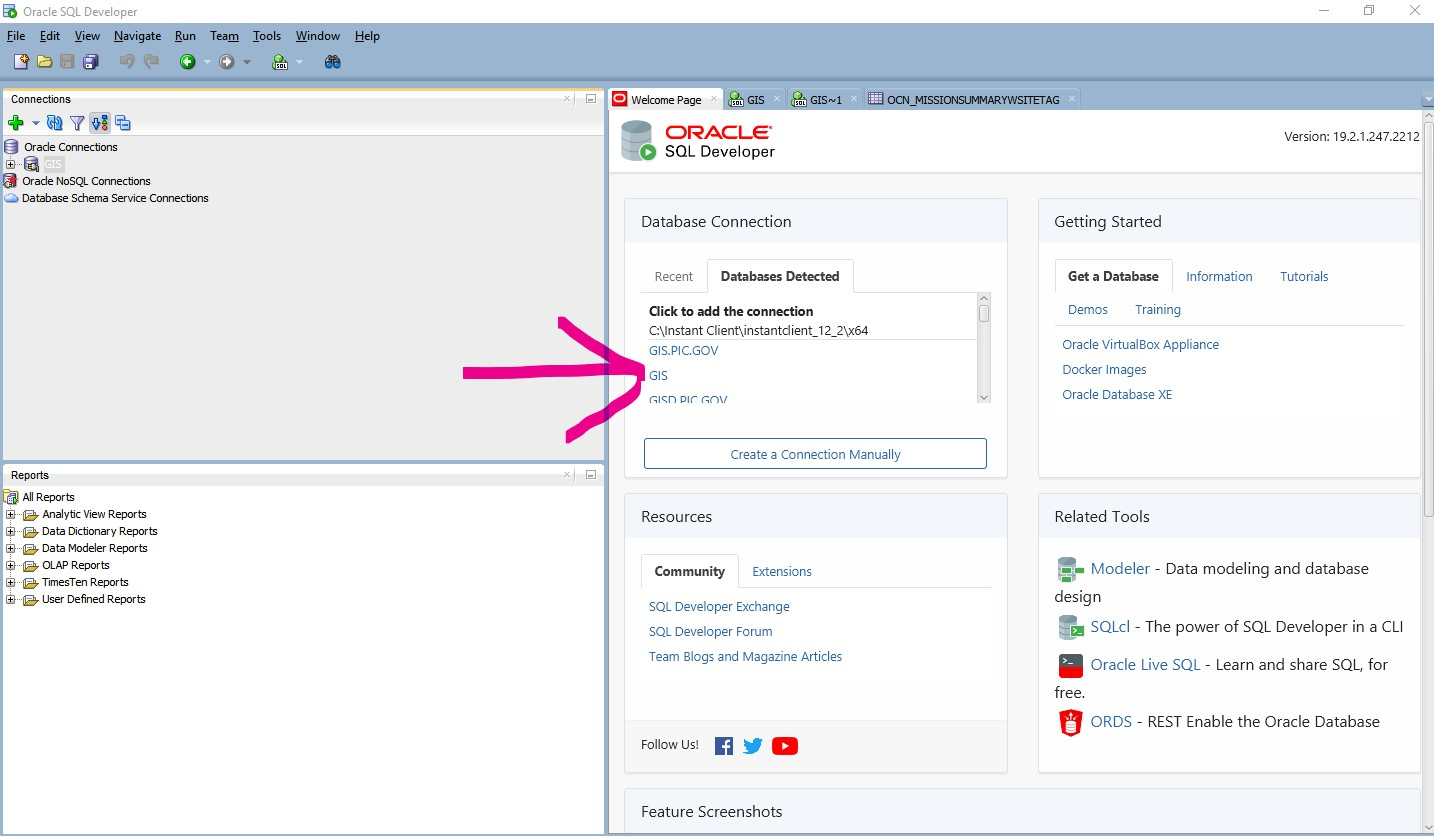
\includegraphics{images/SQL_Dev_Screenshot_1.jpg}
\item
  When prompted, enter your Oracle username and password
  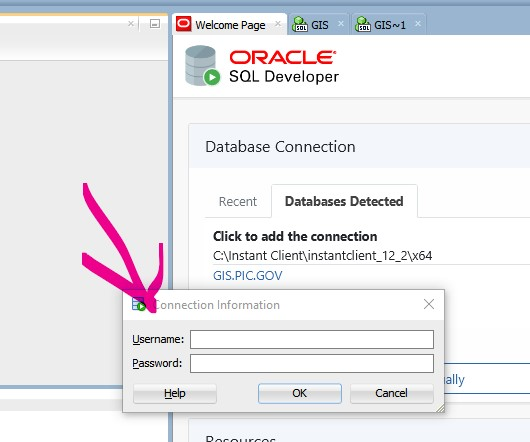
\includegraphics{images/SQL_Dev_Screenshot_2.jpg}
\item
  In the ``Connections'' pane, expand the ``GIS'' database and navigate down to ``Other Users''
  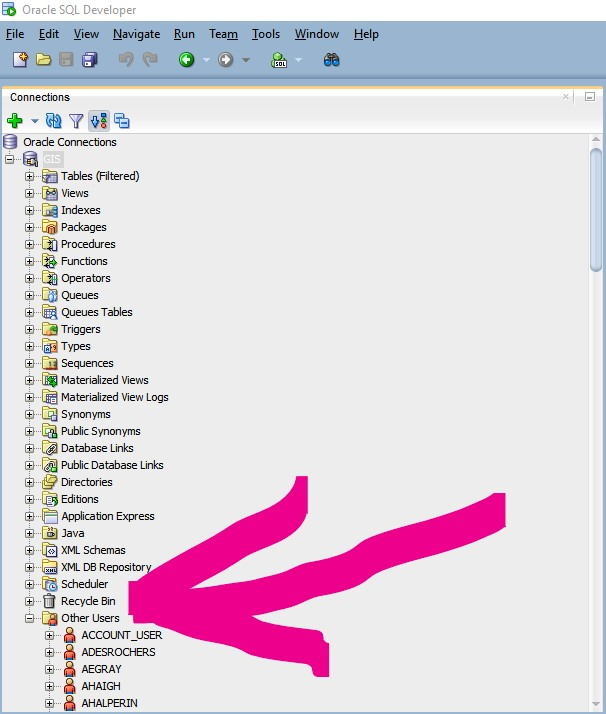
\includegraphics{images/SQL_Dev_Screenshot_3.jpg}
\item
  Expand ``Other Users'' and navigate down to ``GISDAT''
  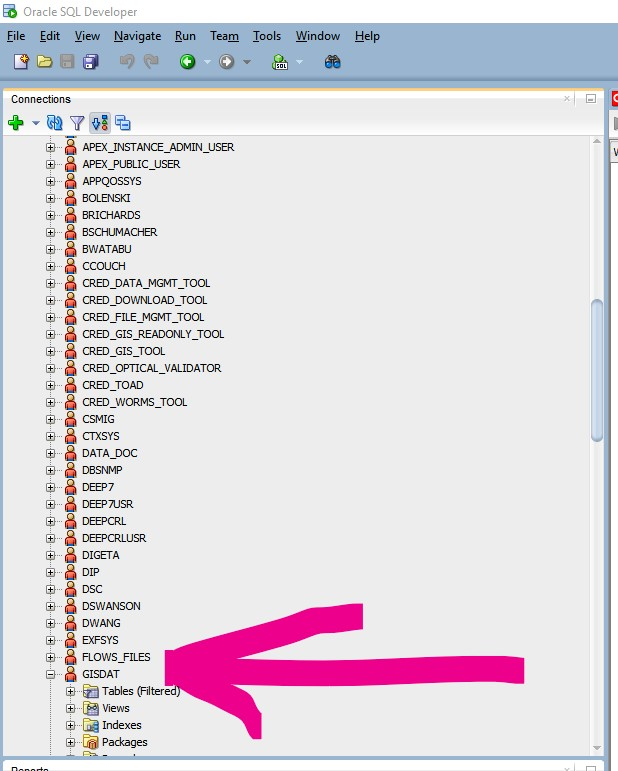
\includegraphics{images/SQL_Dev_Screenshot_4.jpg}
\item
  Within ``GISDAT'' find OCC tables begining with ``OCN'' (note as of March 2020, this is soon to be changed to ``OCC'' prefix when the data team updates the new tables)
\end{enumerate}

\hypertarget{various-underway-resources}{%
\chapter{Various Underway resources}\label{various-underway-resources}}

\textbf{Where to Save Various Data Streams}
Checkout \href{https://docs.google.com/spreadsheets/d/16l1OQgGEunLoADh_MEGyIfbQL2w0u6aw/edit\#gid=1675337307}{this google drive file} showing the paths of where to save various things

\hypertarget{calcification-accretion-unit-cau}{%
\chapter{Calcification Accretion Unit (CAU)}\label{calcification-accretion-unit-cau}}

Authors: Misa PL, Richards CR, Halperin AH, Little AL, and Weible RM (revised March 2020)

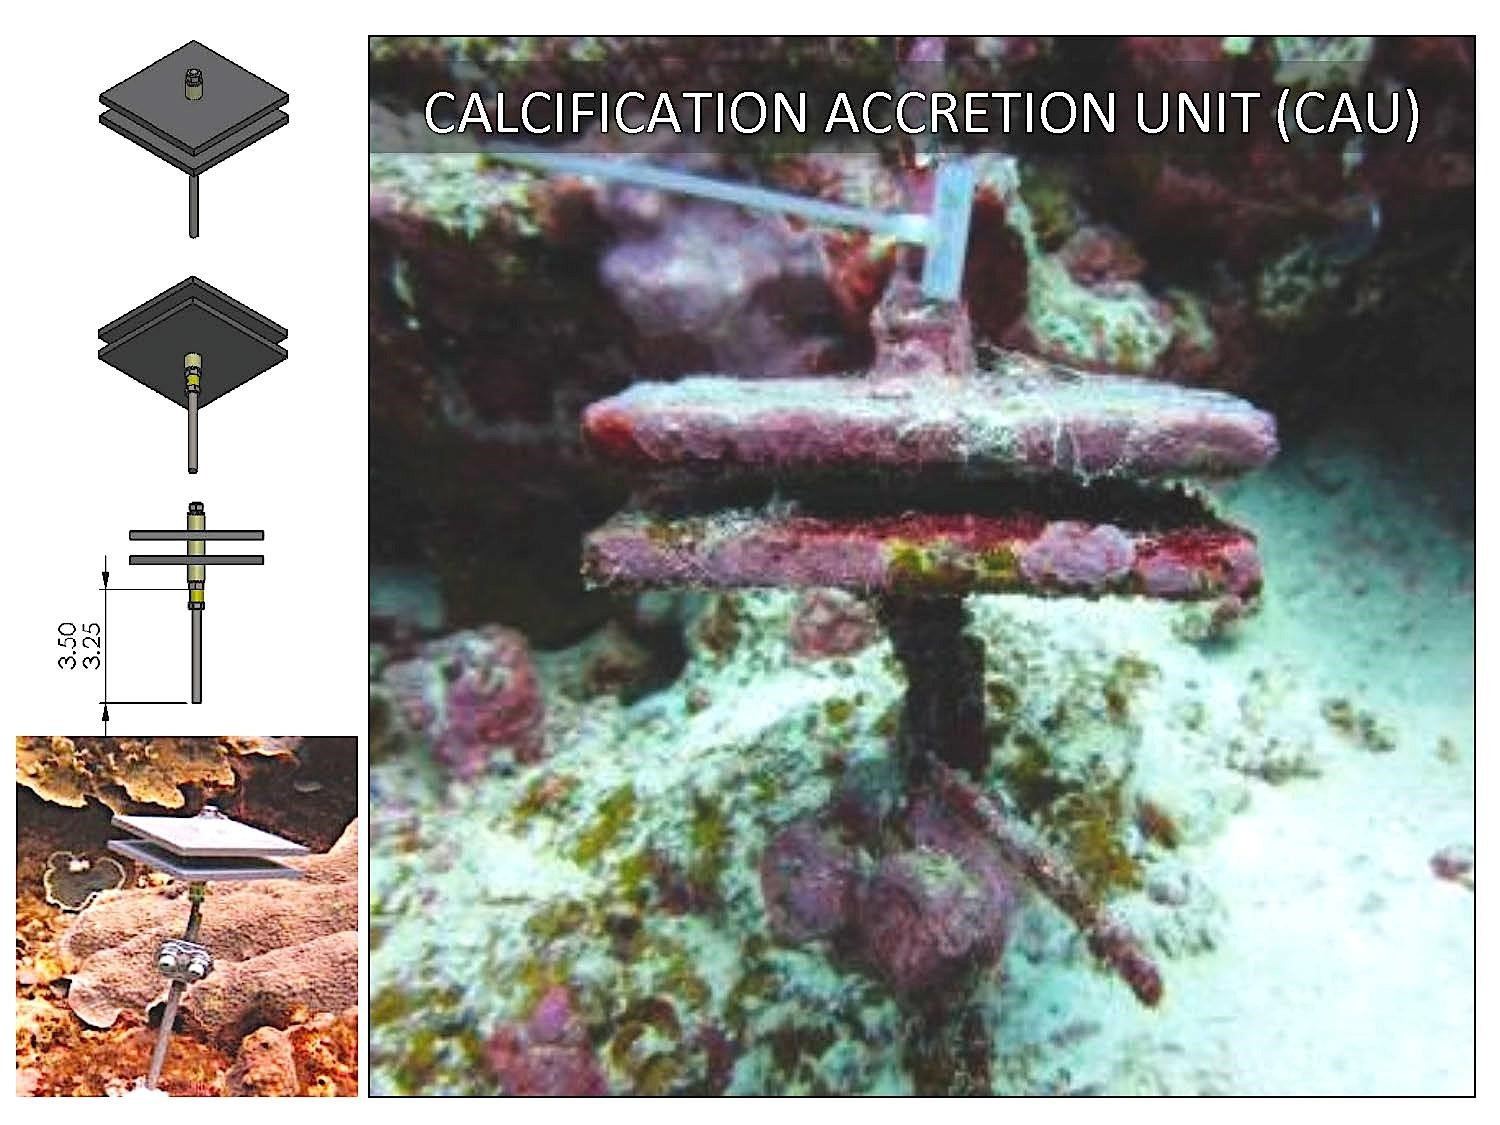
\includegraphics{images/CAU.jpg}

\hypertarget{calcification-accretion-unit-cau-assembly}{%
\section{Calcification Accretion Unit (CAU) Assembly}\label{calcification-accretion-unit-cau-assembly}}

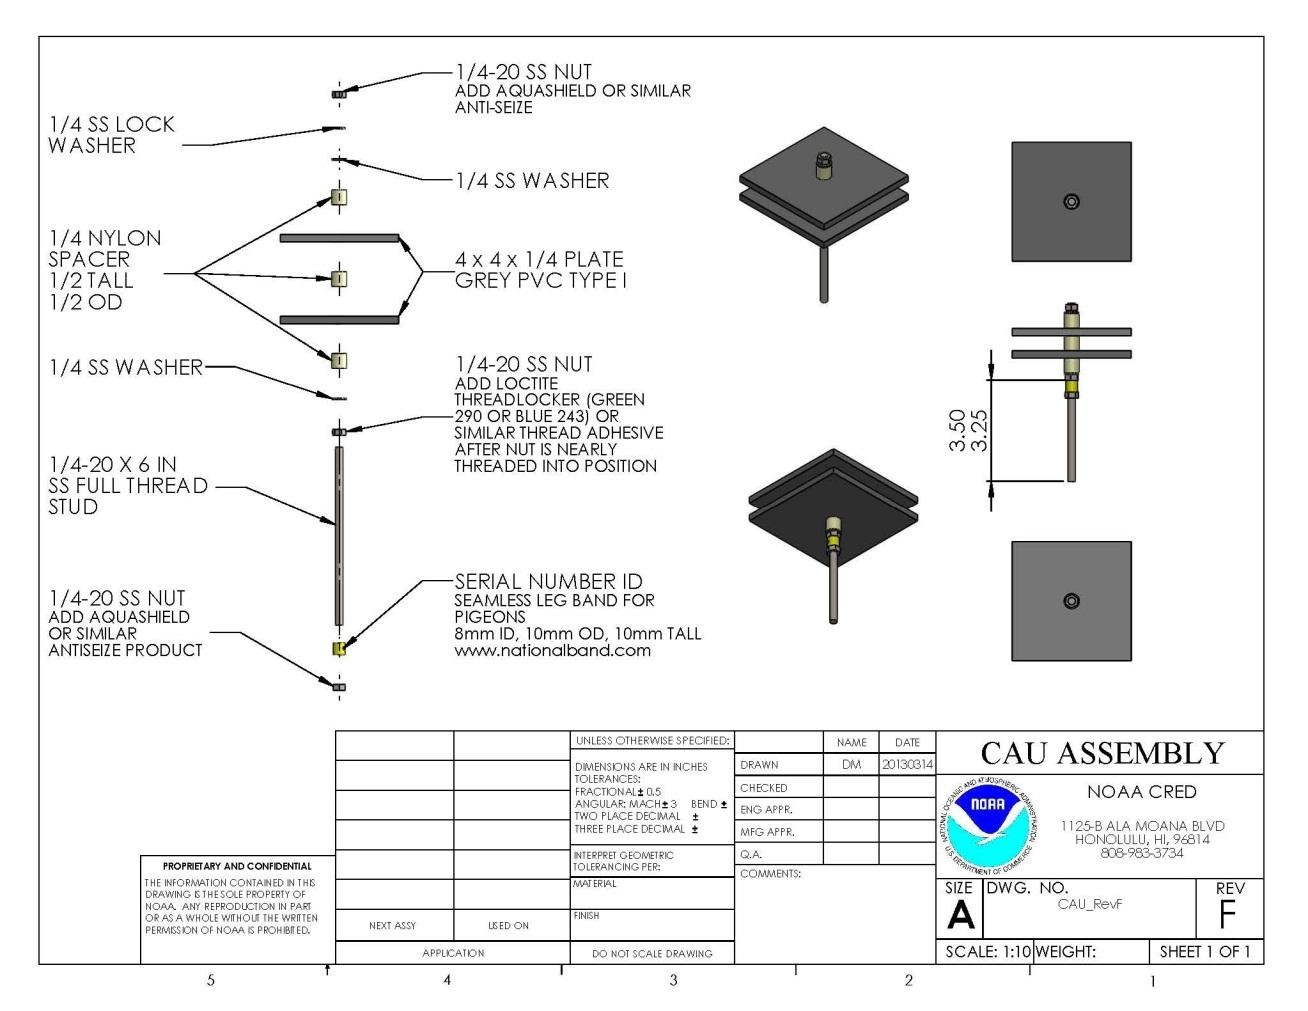
\includegraphics{images/CAU_assembly.jpg}

\hypertarget{calcification-accretion-unit-cau-laboratory-sample-processing-sop}{%
\section{Calcification Accretion Unit (CAU) Laboratory Sample Processing SOP}\label{calcification-accretion-unit-cau-laboratory-sample-processing-sop}}

\hypertarget{preparation-work}{%
\subsection{Preparation Work}\label{preparation-work}}

\textbf{ID Tags}

\begin{enumerate}
\def\labelenumi{\arabic{enumi}.}
\item
  Assign a unique ID to both plates of each Calcification Accretion Unit (CAU) using the \textbf{CAU Plate ID} naming convention SiteID\_RecoveryYear\_4-digitSerial\#\_PlateLocation (``U'' - upper plate, ``L'' - lower plate)

  e.g.~PAL01\_2012\_5319\_U\\
  PAL01\_2012\_5319\_L
\item
  Using a pencil, \textbf{pre-label the following with the CAU Plate ID (e.g.~PAL01\_2012\_5319\_U):}

  \begin{enumerate}
  \def\labelenumii{\alph{enumii})}
  \tightlist
  \item
    Paper tray A - blank index card 12.7 x 20.32cm (5'' x 8'') folded into 12.7 x 12.7cm (5'' x 5'') paper tray\\
  \item
    Paper tray B - same as above\\
  \item
    Filterpaper 11cm diameter, \#1, \textgreater11μm particle retention (e.g.~Whatman No.1001-110)
  \end{enumerate}
\item
  Insert the corresponding Filter paper into the fold of Paper tray B and store in a container. Place Paper tray A in a separate container. Store both containers away from moisture and direct sunlight. See I. Step 8 for pre-weighing instructions.
\item
  Print \textbf{Glass Dish Labels} on waterproof paper using the template in Section VII.C.1. Attach each label on one side of the glass dish with tape.
\item
  Print the Plate Photo ID tags on waterproof paper using the template in Section VII.C.2.There are 4 tags, one for each surface of the CAU to be photographed:

  Upper Plate, Top Side
  Upper Plate, Bottom Side
  Lower Plate, Top Side
  Lower Plate, Bottom Side

  An example of a plate photo ID: \emph{PAL01\_2012\_5319\_U\_T}
\item
  Using an analytical balance, \textbf{pre-weigh} the following and record the value (up to 3 decimal points) in the ESD Apex CAU Mission App (or the CAU Data Entry tool for ESD-CREP users, see Section VI p.~20):

  \begin{enumerate}
  \def\labelenumii{\alph{enumii})}
  \tightlist
  \item
    Paper tray A - record the value in Column (`Paper Tray A Weight {[}g{]}')\\
  \item
    Paper tray B + Filterpaper - record the value in Column (`Filter \& Paper Tray B Dry Weight {[}g{]}')
  \end{enumerate}
\end{enumerate}

\textbf{Re-sealable Bag ID}

Pre-label \textbf{re-sealable plastic bags} 0.95L (1 quart) with the CAU Plate ID. The filter residue will be stored in this bag for archiving

\textbf{Database}

\begin{enumerate}
\def\labelenumi{\arabic{enumi}.}
\item
  Using the \textbf{ESD Apex CAU Mission App} (or the CAU Data Entry tool for ESD-CREP users, see Section VI p.~20), have the Data Management team enter the CAU Site IDs (e.g.~\emph{PAL01}) and 4-digit CAU Serial \#s (e.g.~\emph{5319}) for each unit to be processed
\item
  To calculate the \textbf{``Soak Time''} of each unit, record the CAU ``Deployment Date'' and ``Recovery Date'' in Column CA and CB, respectively. Record any other additional field data in the spreadsheet (e.g.~coordinates, depth, comments, etc.). When using the ESD Apex CAU Mission App, soak time is calculated automatically.
\end{enumerate}

\textbf{Pre-heat Drying Oven}

Oven (Heratherm OGS-180) settings:

\begin{verbatim}
Temperature: 70°C (140°F)  
Damper: level 3 (mid-high)  
\end{verbatim}

\textbf{Prepare 5\% HCl acid solution in 2-liter bottles}

One batch (20-30 units) of CAUs will require about 10-15, 2-liter bottles of 5\% HCl acid solution in order to completely dissolve calcified materials. More may be needed depending on the amount of accreted CaCO3.

To dilute full-strength HCl acid (1.18 g/mL, 36.5 molar mass, 37\% conc.) into 5\% solution, use the recommended ratio below:

\begin{verbatim}
2L stock: 225 ml HCl  
     1775 ml deionized/distilled H2O  

1L stock: 112.5 ml HCl  
     887.5 ml deionized/distilled H2O  
\end{verbatim}

** Be sure to \textbf{ADD ACID TO WATER} to avoid excessive heating, violent boiling or splashing of concentrated acid that could result from the exothermic reaction.
``Do as you oughta, add acid to water!'' - Dr.~Anne Cohen, WHOI

** Acid solutions with a higher (\textgreater5\% HCl concentration) may be prepared and used if desired for processing CAUs from heavily calcified regions (American Samoa, PRIAs), however concentrations \textbf{greater than or equal to 15\% HCl require special PPE including fume hood utilization.}

\hypertarget{cau-processing-steps}{%
\subsection{CAU Processing Steps}\label{cau-processing-steps}}

\emph{see Section IV, p.11 for sample processing timeline and Section VII.A, p.36 for sample daily task guide}

\hypertarget{dissassembling-and-photo-documentation}{%
\subsubsection{Dissassembling and Photo-documentation}\label{dissassembling-and-photo-documentation}}

\begin{enumerate}
\def\labelenumi{\arabic{enumi}.}
\item
  Thaw a batch of CAUs (typically 20-30 units) in the sink for at least 12 hours. Do not thaw over water.
\item
  Disassemble the plates of each CAU by removing the hex nuts and washers using two 1/4" wrenches (one to hold the unit steady). Make sure to maintain plate identity (upper vs lower plate, top vs bottom side of plate) and the CAU Plate ID.
\end{enumerate}

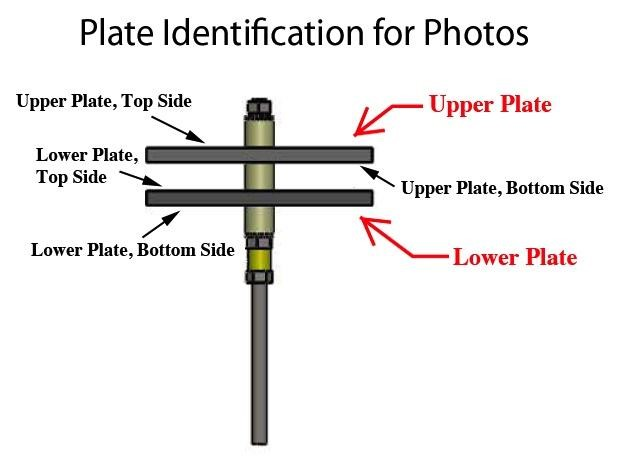
\includegraphics{images/CAU_plate_ID.jpg}

\begin{enumerate}
\def\labelenumi{\arabic{enumi}.}
\setcounter{enumi}{2}
\item
  Carefully rinse each plate in a saltwater rinse basin (if saltwater is not readily available, freshwater may be used) to remove loose sediment, sand and mobile fauna. Discard any mobile fauna that may have fallen off during rinsing.
\item
  Fill each pre-labeled glass dish with saltwater(or freshwater).
\item
  Place each CAU plate with the \textbf{top plate facing upwards} into its corresponding glass dish. Ensure that the plate and any encrusting fauna are completely submerged in water. Add more water if necessary (see Section V.C for additional instructions)
\end{enumerate}

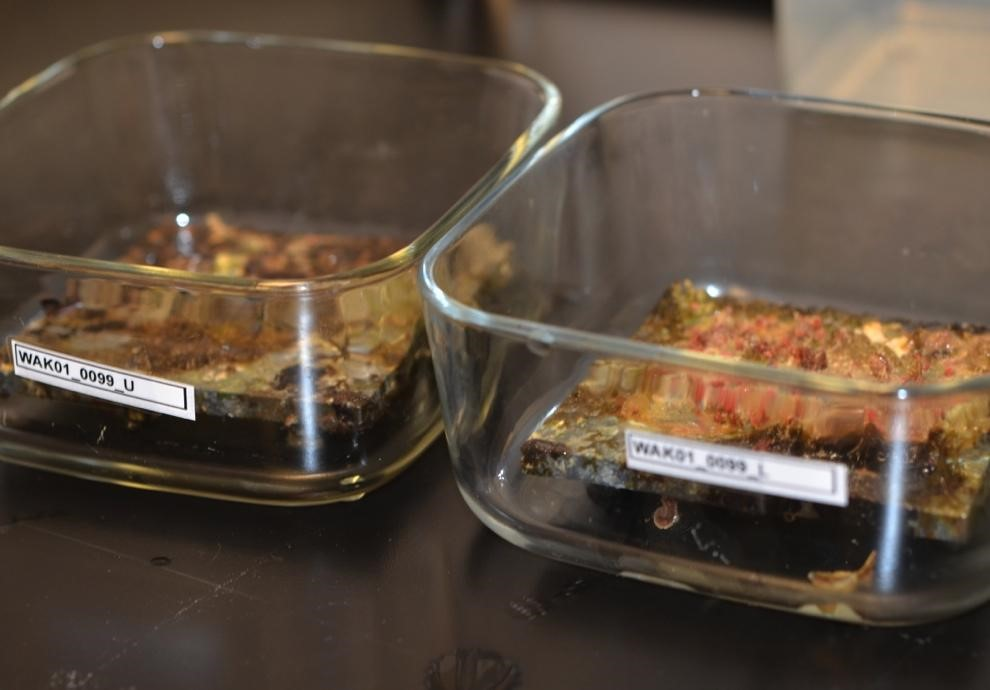
\includegraphics{images/CAU_dried.jpg}

\begin{enumerate}
\def\labelenumi{\arabic{enumi}.}
\setcounter{enumi}{5}
\tightlist
\item
  Attach a DSLR camera to a camera copy stand or a tripod. Arrange lighting such that the plate is fully illuminated and no glare is visible to the camera
\end{enumerate}

** \emph{If using a Nikon D7000 camera mounted on a copy stand kit with attached lights, see Section V, p.~12 for tethering protocol and recommended settings (\textbf{f/8, ISO400, AWB}).}

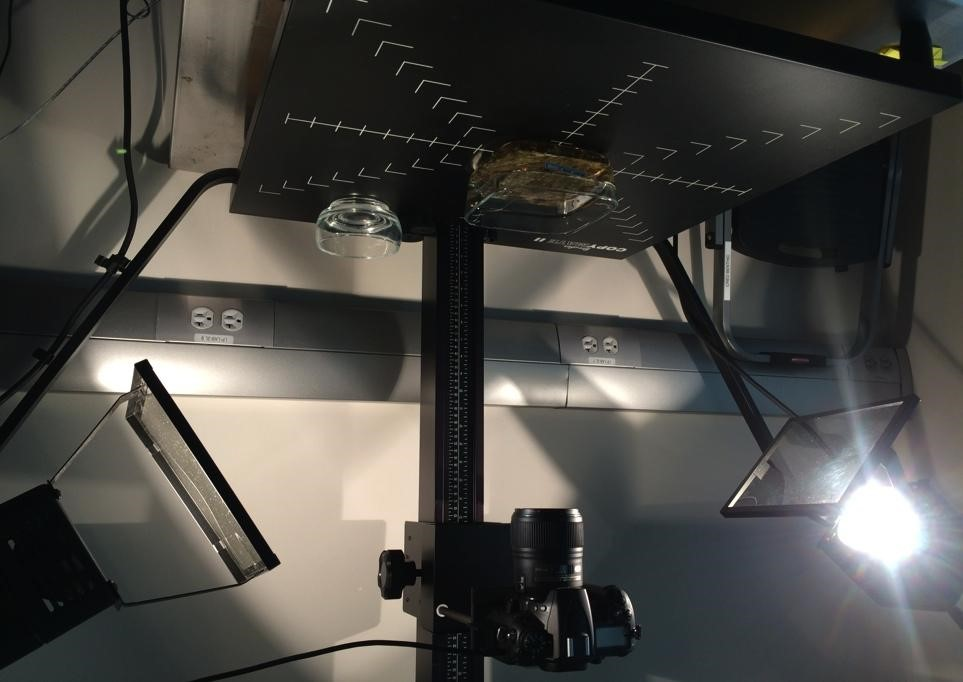
\includegraphics{images/CAU_photograph.jpg}

\begin{enumerate}
\def\labelenumi{\arabic{enumi}.}
\setcounter{enumi}{6}
\tightlist
\item
  It is recommended to tether the camera to a computer and save the photos directly to the computer's local drive (while using the camera's SD card as a backup drive). Designate a folder where the CAU photoset will be stored directly.
\end{enumerate}

(May 2019 - ESD General (T:) Drive at:

\begin{verbatim}
T:\\Oceanography\\CAUs\\Analysis
\end{verbatim}

organized by Year and Cruise Mission, or Island Code for shore-based missions or those from the Atlantic.)

\begin{enumerate}
\def\labelenumi{\arabic{enumi}.}
\setcounter{enumi}{7}
\tightlist
\item
  Photograph the top and bottom of each plate, first with the Plate Photo ID tag and then a 2nd image without the tag. (If pieces of calcified material fall off during the photographing process, retain the pieces with the plate to be used during the decalcification process).
\end{enumerate}

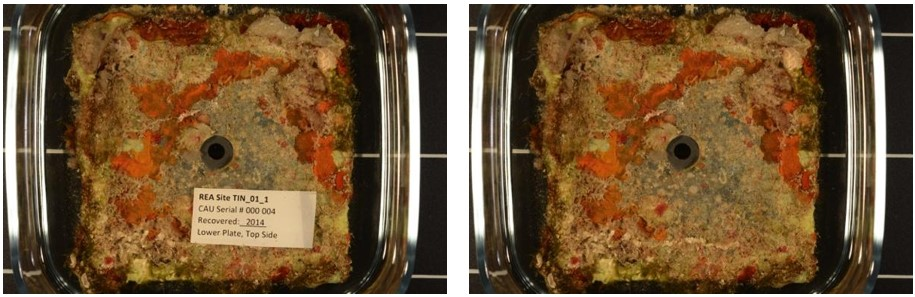
\includegraphics{images/CAU_image.jpg}

\begin{enumerate}
\def\labelenumi{\arabic{enumi}.}
\setcounter{enumi}{8}
\item
  From the designated CAU photoset folder, confirm that both plate photos (with and without the Plate Photo ID tag) are in focus. After photographing both sides of each plate, each CAU photoset folder should have \textbf{8 photos}. The photos should be later on renamed with the following naming convention:

  \textbf{a) With Plate Photo ID tag:}\\
  *SiteID\_RecoveryYear\_4-digitSerial\#\_PlateLocation (``U'' - upper plate or ``L'' - lower plate)\_PlateSurface (``T'' - top plate or ``B'' - bottom plate)\_ID.jpg*

  \textbf{b) Without Plate Photo ID tag:}\\
  *SiteID\_RecoveryYear\_4-digitSerial\#\_PlateLocation (``U'' - upper plate, ``L'' lower plate)\_PlateSurface (``T'' - top plate, ``B'' - bottom plate).jpg*

  Example:
  PAL01\_2012\_5319\_U\_T\_ID.jpg -- Upper Plate, Top Side with tag\\
  PAL01\_2012\_5319\_U\_T.jpg -- Upper Plate, Top Side\\
  PAL01\_2012\_5319\_U\_B\_ID.jpg -- Upper Plate, Bottom Side with tag
  PAL01\_2012\_5319\_U\_B.jpg -- Upper Plate, Bottom Side\\
  PAL01\_2012\_5319\_L\_T\_ID.jpg -- Lower Plate, Top Side with tag\\
  PAL01\_2012\_5319\_L\_T.jpg -- Lower Plate, Top Side\\
  PAL01\_2012\_5319\_L\_B\_ID.jpg -- Lower Plate, Bottom Side with tag\\
  PAL01\_2012\_5319\_L\_B.jpg -- Lower Plate, Bottom Side
\item
  After photographing all units, if the CAUs were submerged in seawater, carefully rinse each plate in freshwater. If the CAUs were submerged in freshwater, skip the rinsing process.
\item
  Be sure to remove all hex nuts and washers that may still be attached at the center of the plate. Hex nuts and washers can be covered by calcified material and difficult to see. Inspect each side of each plate to ensure that there are no washers or hex nuts present. If a hex nut or washer is covered in calcified material, remove the hardware and chip off the calcified material from the hardware. Retain the removed material with the rest of the plate.
\item
  Place each plate and any dislodged pieces of calcified material on its corresponding Paper Tray A, then onto a drying rack and placed in the fume hood. The drying rack can be left in a fume hood to air dry at room temperature indefinitely (\textbf{minimum of 24 hours}), until they are dried in the oven.
\end{enumerate}

Drying at room temperature before placing in the oven can help reduce the time the plates remain in the oven.

Wash and rinse the glass dishes but keep the labels on. The same glass dishes will be used during the HCl acid decalcification process.

\hypertarget{determining-the-weight-of-the-cau-plate}{%
\subsubsection{Determining the weight of the CAU plate}\label{determining-the-weight-of-the-cau-plate}}

\begin{enumerate}
\def\labelenumi{\arabic{enumi}.}
\tightlist
\item
  After a minimum air-drying period of 24 hours, place the \textbf{plate assembly (plate, dislodged pieces of calcified material and Paper Tray A)} in the oven labeled ``\textbf{Non-HCl}'' to dry at 60°C for 24 hours.
\end{enumerate}

** \emph{Check that the internal temperature remains consistent. If not, minor adjustments should be made to the oven temperature and damper settings.}

\begin{enumerate}
\def\labelenumi{\arabic{enumi}.}
\setcounter{enumi}{1}
\item
  After 24 hours, remove the plate assembly and allow it to come to room temperature (roughly 10 min).
\item
  Weigh the \textbf{entire plate assembly}.
\item
  In the ESD Apex CAU Mission App (or CAU Data Entry tool for ESD-CREP users), record the weight to at least 3 decimal places under the column `\emph{Drying 1 {[}24 h{]} {[}paper tray + CAU plate{]} {[}g{]}}'.
\item
  Return the plate assembly in the oven.
\item
  Dry the CAU plates for another 24 hours.
\item
  Remove the plate assembly and allow it to come to room temperature (roughly 10 min).
\item
  Weigh the \textbf{entire plate assembly}.
\item
  In the ESD Apex CAU Mission App (or CAU Data Entry tool for ESD-CREP users), record the 2nd weight to at least 3 decimal places under the column `\emph{Drying 2 {[}48 h{]} {[}paper tray + CAU plate{]} {[}g{]}}'.
\item
  Compare the current weight from the previous weight:
\end{enumerate}

\begin{itemize}
\item
  If the difference in weight is less than 0.1g, the plates are considered dry and no further drying needs to occur. This is automatically calculated by the ESD Apex CAU Mission App and denoted by the `Plate Dry' column on the far right saying `YES'.
\item
  If the difference in weight is greater than 0.1 g, return the plates to the oven for another 24 hours.
\end{itemize}

\begin{enumerate}
\def\labelenumi{\arabic{enumi}.}
\setcounter{enumi}{10}
\tightlist
\item
  Repeat \emph{III.B Steps 5-10} until the difference in weight is less than 0.1 g.
\end{enumerate}

\hypertarget{decalcification-of-caco3-in-hydrochloric-acid}{%
\subsubsection{Decalcification of CaCO3 in Hydrochloric Acid}\label{decalcification-of-caco3-in-hydrochloric-acid}}

\textbf{Be sure to wear proper PPE when handling acid contaminated objects (steps 1-9) including gloves, safety glasses, and lab coat.}

\begin{enumerate}
\def\labelenumi{\arabic{enumi}.}
\item
  Ensure that the plate is fully dry (mass lost between last two weighing will have been less than 0.1g) and the weight of the plate assembly and Paper Tray A has been recorded.
\item
  Place the individual plates in the pre-labeled glass dishes. Keep Paper Tray A and place under the glass dish.
\item
  Chip off large pieces of calcified materials (e.g.~CCA, coral, shells, etc.) and grind using a mortar and pestle. Return the pulverized forms in the glass dish.
\item
  Fill the glass dish midway with 5\% HCl (or otherwise chosen concentration) acid solution or until the entire CAU plate is fully submerged in acid. \textbf{Add HCl acid slowly as the solution may overflow when bubble formation/decalcification begins. The overflow most definitely occurs when dissolving plates from Rose and Swains Atoll.}
\item
  When decalcification has slowed (12-24 hours):
\end{enumerate}

\begin{itemize}
\item
  Scrape leftover material from the CAU plates with a razor blade into the glass dish. (See III.C, Step 8-15).
\item
  Grind pieces of calcified materials that may still be present and return in the glass dish.
\item
  Using acid-resistant gloves, sort through the scraped fleshy material in the glass dish and feel for any calcified materials.
\item
  Some calcified material can be completely covered by a boundary layer of fleshy material. If present, manually tease the fleshy material and grind the calcified material to allow decalcification to continue.
\item
  If there are more calcified materials in the dish, but no obvious decalcification occurring (no bubble formation), decant the used acid solution and drain the fleshy material into another pre-labeled containers (beakers, glass dish, etc). Add new 5\% HCl acid solution (*or desired concentration) in the first glass dish to continue dissolving the remaining calcified materials.
\end{itemize}

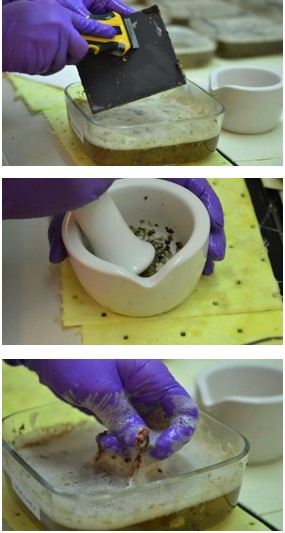
\includegraphics{images/CAU_dissolve.jpg}

\begin{enumerate}
\def\labelenumi{\arabic{enumi}.}
\setcounter{enumi}{5}
\item
  Repeat III.C, Steps 5b)-e) until all CaCO3 is fully dissolved. Additional 5\% HCl acid solution (*or desired concentration) may need to be added 2-4x, depending on the amount of CaCO3 present.
\item
  Using 5\% HCl acid (*or desired concentration) in a squeeze bottle, thoroughly rinse the tools (gloves, mortar and pestle, razor/scraper) into the glass dish.
\item
  When the CAU PVC plates have been scraped clean (fleshy/calcified material completely removed from either side and edges of the plate), rinse all sides of the plates with 5\% acid (*or desired concentration) into the glass dish.
\item
  Have a bowl of freshwater ready to scrub and rinse the CAU PVC plates once they are completely clear of particles from the previous step. Pat to dry.
\item
  Place the CAU PVC plate on its corresponding Paper Tray A.
\item
  Place the rinsed CAU PVC plates in the oven at 60°C for 24 hours on top of the corresponding Paper Tray A.
\item
  Remove the plate from the oven and allow to come to room temperature (roughly 10 min).
\end{enumerate}

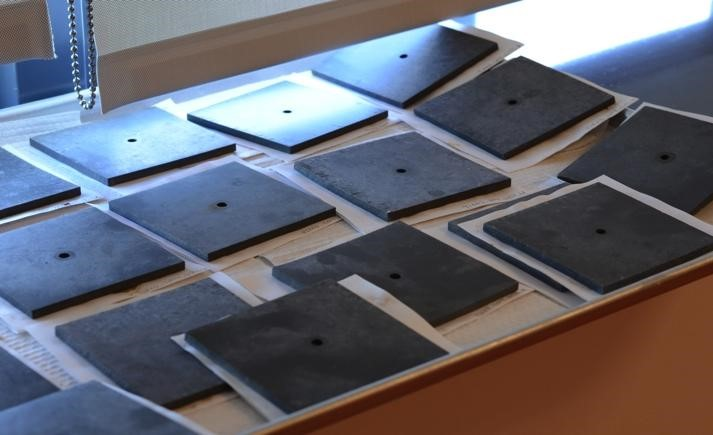
\includegraphics{images/CAU_drying.jpg}

\begin{enumerate}
\def\labelenumi{\arabic{enumi}.}
\setcounter{enumi}{12}
\item
  Weigh the clean and dry CAU PVC plate without the underlying paper tray. - *Paper Tray A can be discarded after the CAU PVC plates have been weighed and recorded.
\item
  In the ESD Apex CAU Mission App, record the weight to at least 3 decimal places under the column `\emph{CAU PVC Dry Weight {[}g{]}}'.
\item
  Collect the clean and weighed CAU PVCs and store for redeployment/archiving.
\end{enumerate}

\hypertarget{vacuum-filtration-of-fleshy-material}{%
\subsubsection{Vacuum filtration of fleshy material}\label{vacuum-filtration-of-fleshy-material}}

\textbf{Be sure to wear proper PPE when handling acid contaminated objects (steps 1-4) including gloves, safety glasses, and lab coat.}

\begin{enumerate}
\def\labelenumi{\arabic{enumi}.}
\item
  Using a 4-liter Buchner funnel, a plastic mesh layer (with attached pull string) and the corresponding pre-weighed filter paper, vacuum filter the acid bath and remaining fleshy material for each CAU plate. Use a freshwater squeeze bottle to rinse contents of the glass dish into the funnel.
\item
  If the volume of fleshy material is sufficient to clog the filter paper, a 2nd pre-labeled and pre-weighed filter paper (\emph{see III.D, Step 2, a-c}) can be used to filter the remaining volume of acid bath and fleshy material:
\end{enumerate}

\begin{itemize}
\item
  Label an additional filter paper and paper tray with its corresponding CAU Plate ID (e.g.~\emph{PAL01\_2012\_5319\_U}).
\item
  In the ESD Apex CAU Mission App, record the weight of the 2nd filter paper + paper tray to at least 3 decimal places in the column `\emph{Addtl Filter \& Paper tray B Dry Weight {[}g{]}}'.
\end{itemize}

\begin{enumerate}
\def\labelenumi{\arabic{enumi}.}
\setcounter{enumi}{2}
\tightlist
\item
  If filtering has slowed down, use a spatula/teaspoon to gently scrape the surface of the filter paper to allow more solution to filter through. Filtering can take \textgreater5 mins depending the amount of fleshy material in the acid bath.
\end{enumerate}

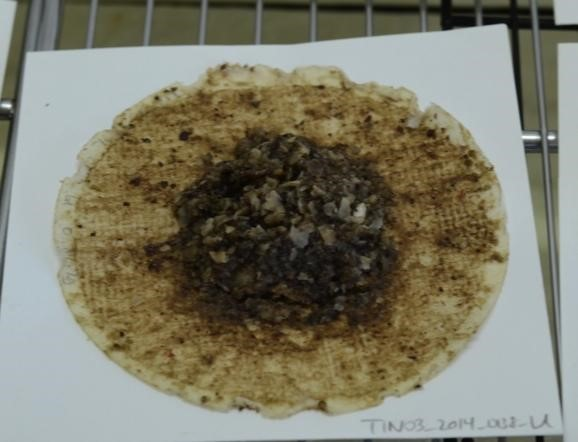
\includegraphics{images/CAU_filter.jpg}

\begin{enumerate}
\def\labelenumi{\arabic{enumi}.}
\setcounter{enumi}{3}
\tightlist
\item
  When filtration is completed, place the filter paper on its corresponding Paper Tray B and onto a drying rack. The drying rack should be left in a fume hood to air dry at room temperature (minimum of 24 hours). The filter paper can continue to air dry at room temperature, indefinitely, until they are dried in the oven.
\end{enumerate}

\hypertarget{determining-the-weight-of-the-fleshy-material}{%
\subsubsection{Determining the weight of the fleshy material}\label{determining-the-weight-of-the-fleshy-material}}

\textbf{Be sure to wear proper PPE (gloves) when handling acid contaminated filters in this section.}

\begin{enumerate}
\def\labelenumi{\arabic{enumi}.}
\tightlist
\item
  After a minimum air-drying period of 24 hours, place the \textbf{filter paper assembly (filter paper and Paper Tray B)} in the oven to dry at 60°C for 24 hours.
\end{enumerate}

** \emph{Check that the internal temperature remains consistent. If not, minor adjustments should be made to the oven temperature and damper settings.}

\begin{enumerate}
\def\labelenumi{\arabic{enumi}.}
\setcounter{enumi}{1}
\item
  After 24 hours, remove the filterpaper assembly and allow it to come to room temperature (roughly 10min).
\item
  Weigh the \emph{entire filterpaper assembly.}
\end{enumerate}

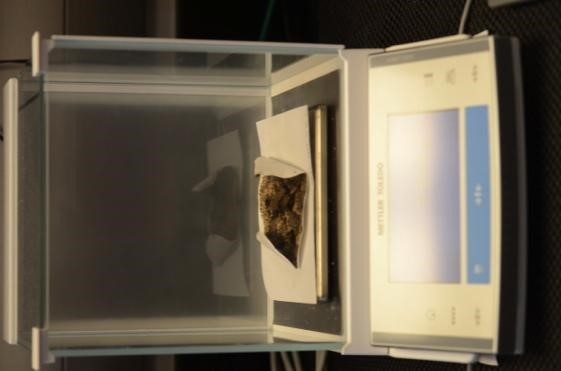
\includegraphics{images/CAU_weigh.jpg}

\begin{enumerate}
\def\labelenumi{\arabic{enumi}.}
\setcounter{enumi}{3}
\item
  In the ESD Apex CAU Mission App, record the weight to at least 3 decimal places under ``Filters'' \textgreater{}`\emph{Drying 1 {[}24 h{]} {[}paper tray + filterpaper{]} {[}g{]}}'.
\item
  Return the filterpaper assembly to the oven.
\item
  Dry the filterpaper for another 24 hours.
\item
  Remove the filterpaper assembly and allow it to come to room temperature (roughly 10min).
\item
  Weigh the \textbf{entire filterpaper assembly}
\item
  In the ESD Apex CAU Mission App, record the weight to at least 3 decimal places under ``Filters'' \textgreater{}`\emph{Drying 2 {[}48 h{]} {[}paper tray + filterpaper{]} {[}g{]}}'.
\item
  Compare the current weight from the previous weight:
\end{enumerate}

\begin{itemize}
\tightlist
\item
  If the difference in weight is less than 0.1g, the plates are considered dry and no further drying/weighing needs to occur.
\end{itemize}

** \emph{In the ESD Apex CAU Mission App, the column to the far right called ``Filter Dry'' has been formatted to change from `NO' to ``YES'' if the difference in weight is less than 0.1g.}

\begin{itemize}
\tightlist
\item
  If the difference in weight is greater than 0.1 g, return the plates to the oven for another 24 hours.
\end{itemize}

\begin{enumerate}
\def\labelenumi{\arabic{enumi}.}
\setcounter{enumi}{10}
\item
  Repeat III.E Steps 5-10 until the difference in weight is less than 0.1 g.
\item
  After recording the final filterpaper assembly dry weight, place the filterpaper and Paper tray B in its corresponding re-sealable bag for archiving. Ensure the bag is labeled properly using the CAU Plate ID naming convention:
\end{enumerate}

*SiteID\_RecoveryYear\_4-digitSerial\#\_PlateLocation (``U'' - upper plate, ``L'' - lower plate)*

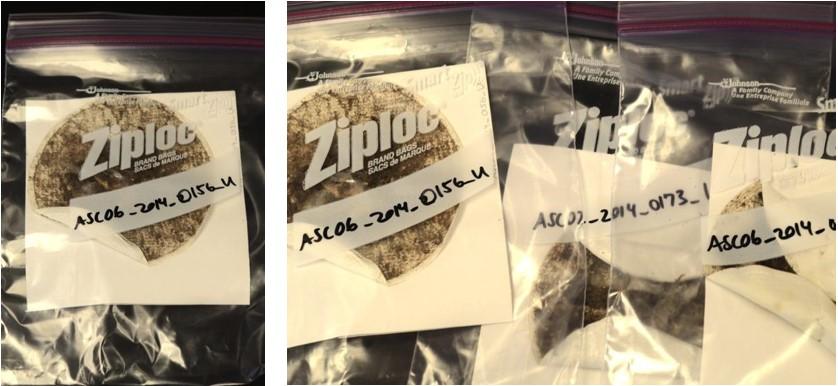
\includegraphics{images/CAU_bag.jpg}

\hypertarget{processing-timeline}{%
\subsection{Processing Timeline}\label{processing-timeline}}

Approximately 25 units or 50 CAU plates can be processed as a batch (at ESD-CREP, this is equivalent to CAUs collected from about 1 island). The processing of each batch is typically completed in 4 weeks. Below is an example of a typical processing timeline

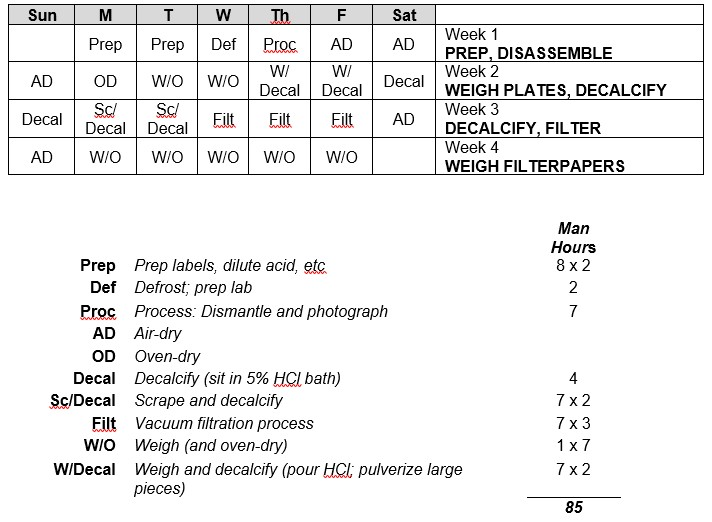
\includegraphics{images/CAU_table.jpg}

\hypertarget{camera-tethering-and-cau-plate-photo-documentation-via-nikon-camera-control-pro-2}{%
\subsection{Camera tethering and CAU plate photo-documentation via Nikon Camera Control Pro 2}\label{camera-tethering-and-cau-plate-photo-documentation-via-nikon-camera-control-pro-2}}

\emph{Refer to the brand/model user documentation/manual if using a different camera and setup}

\hypertarget{installing-the-software}{%
\subsubsection{Installing the software}\label{installing-the-software}}

For ESD-CREP users, the installation instructions and software product key can be accessed in the network folder

\begin{verbatim}
T:\\general\\ProjectGroup\\Ocean Acidification\\CAUs\Analysis\\CAU Processing SOP, Data sheet, Labels\\CAU SOPs 2015\\CAUSOP_NikonD7000Settings.pdf
\end{verbatim}

\hypertarget{connecting-the-camera-to-the-computer}{%
\subsubsection{Connecting the camera to the computer}\label{connecting-the-camera-to-the-computer}}

\begin{enumerate}
\def\labelenumi{\arabic{enumi}.}
\tightlist
\item
  Connect Nikon DSLR camera (Nikon D7000 with AF-S Micro NIKKOR 60mm f\textbackslash2.8G ED lens) to the computer via USB mini cable
\end{enumerate}

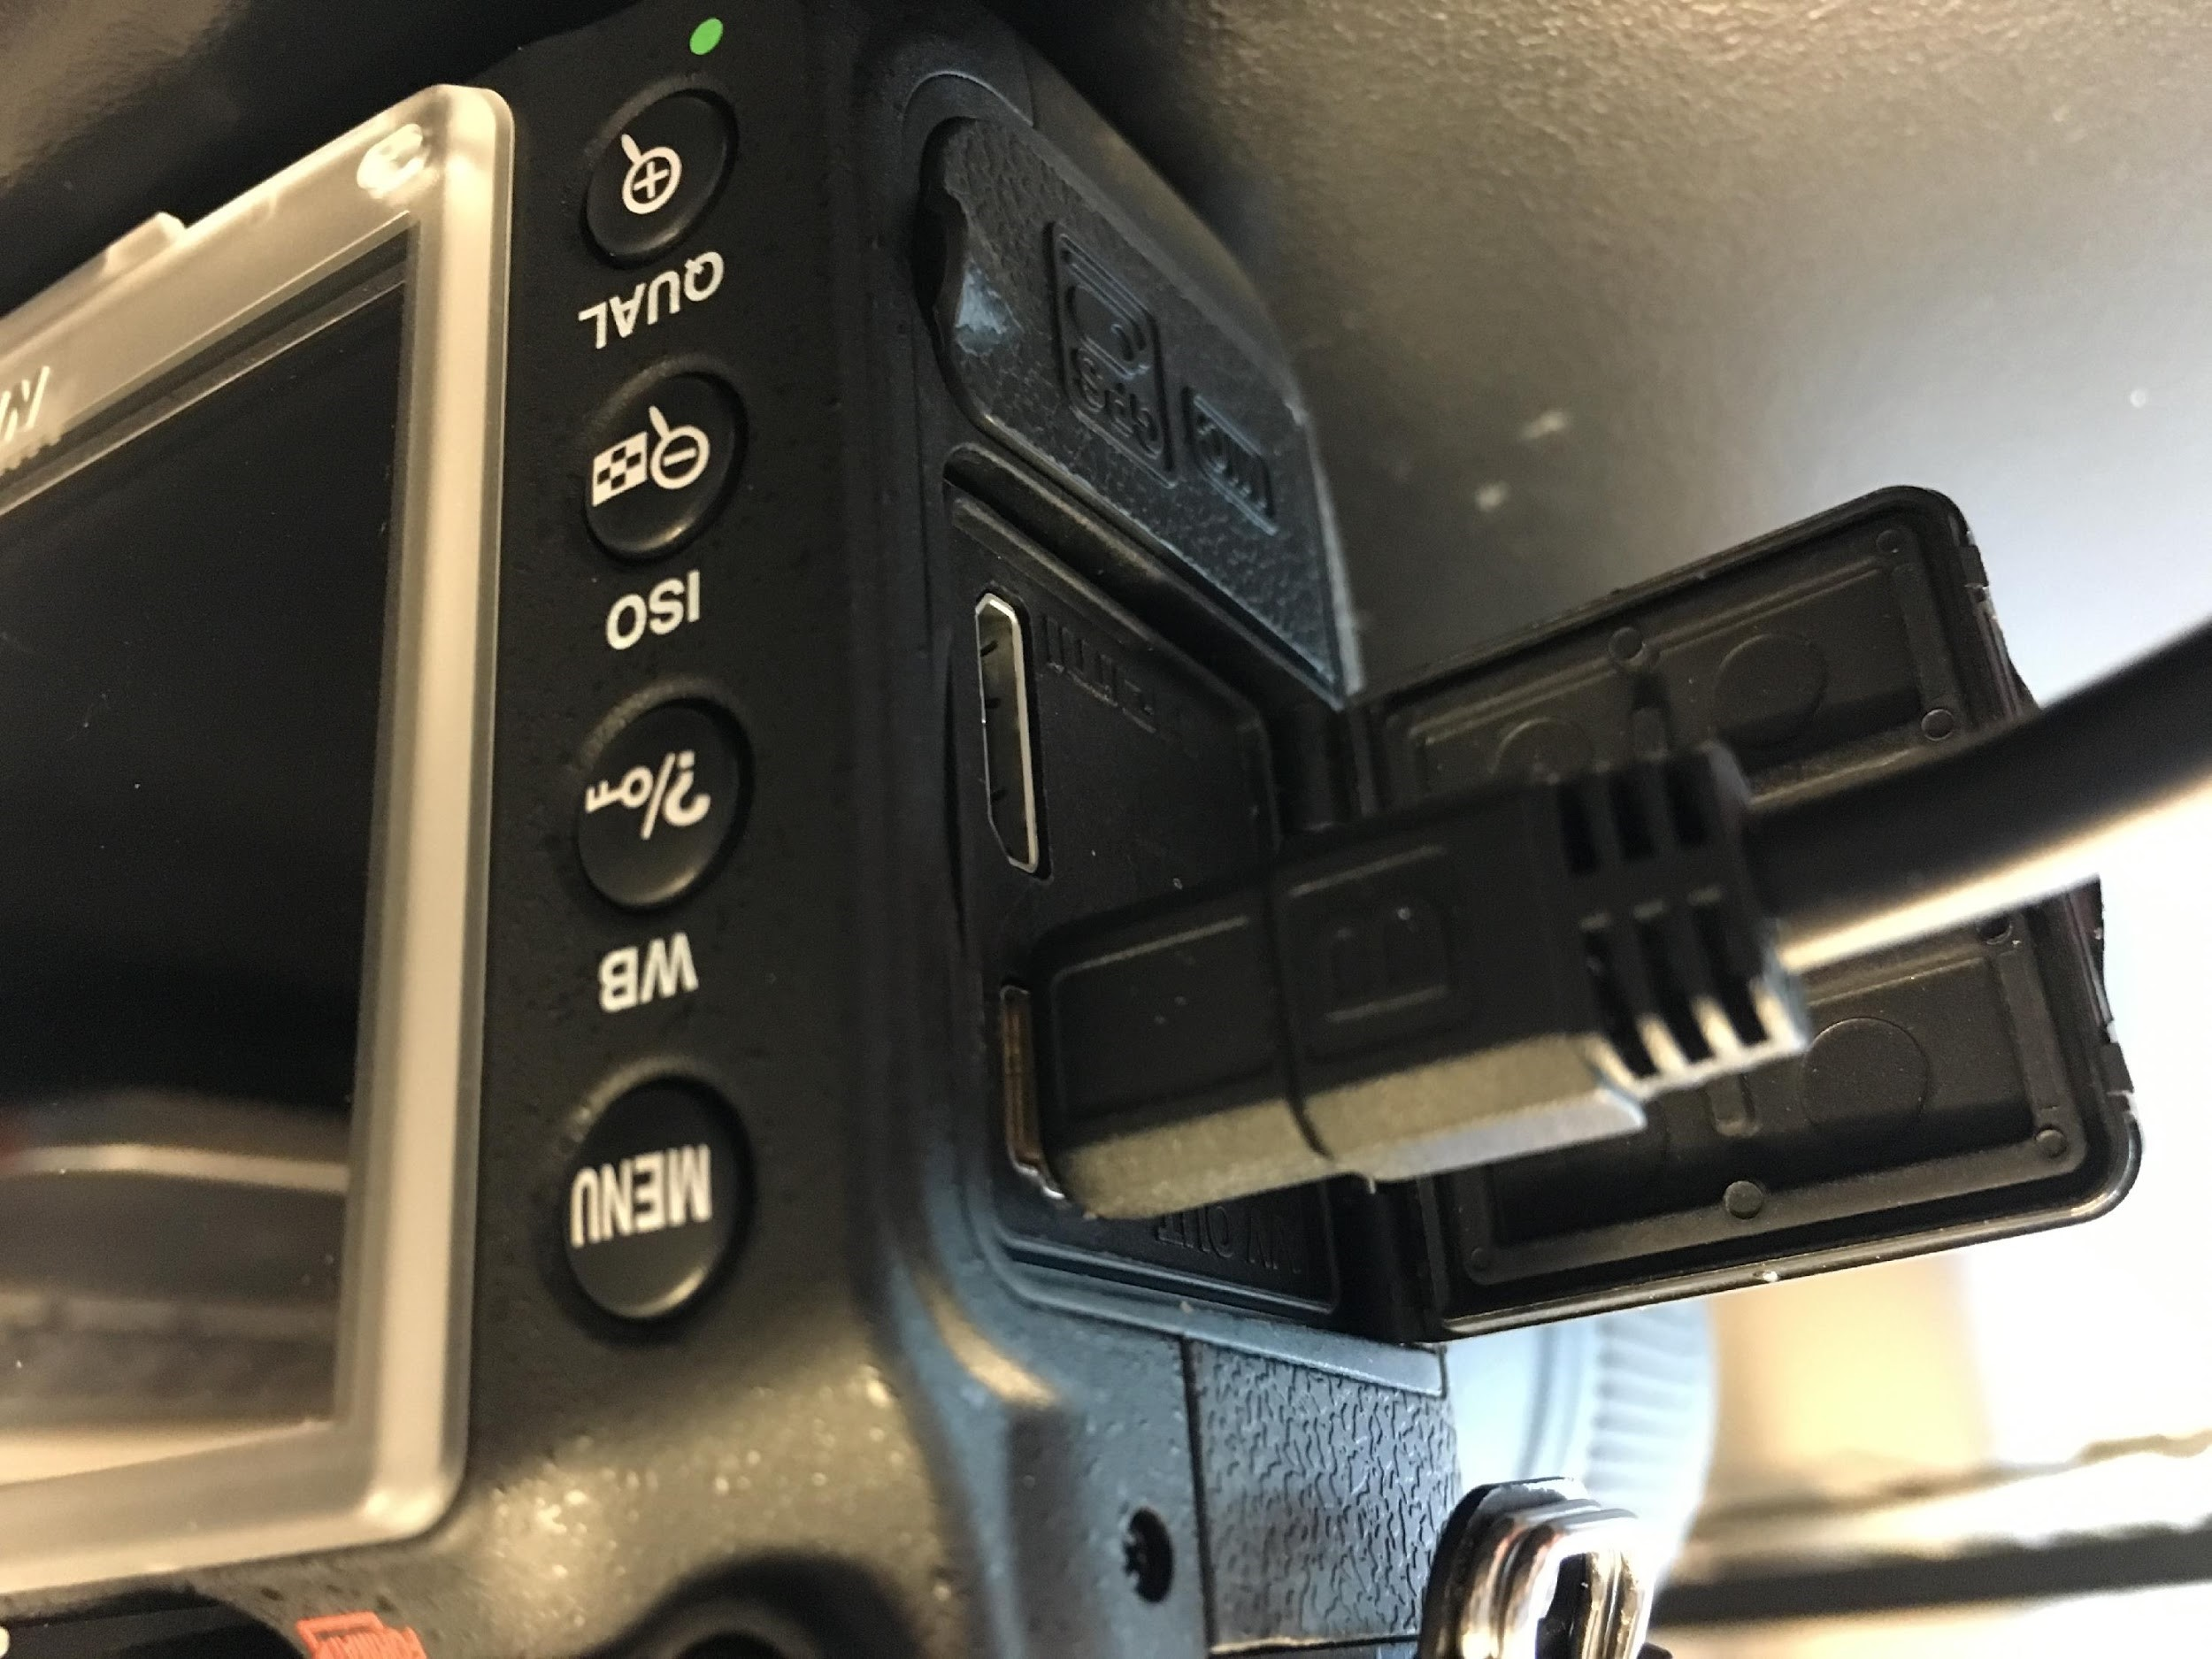
\includegraphics{images/Camera.jpg}

\begin{enumerate}
\def\labelenumi{\arabic{enumi}.}
\setcounter{enumi}{1}
\item
  Start the Nikon Camera Control Pro 2 application
\item
  Turn the camera ON
\item
  Once connected, the connection status of the camera in use will be displayed on the Camera Control Pro window
\end{enumerate}

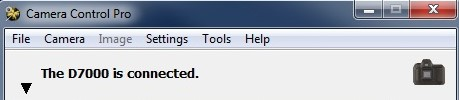
\includegraphics{images/Camera2.jpg}

\begin{enumerate}
\def\labelenumi{\arabic{enumi}.}
\setcounter{enumi}{4}
\tightlist
\item
  \textbf{If using the software for the FIRST TIME:}
\end{enumerate}

\begin{itemize}
\item
  Click on ``\textbf{Exposure 1}'' under the Camera Control tabs and change the settings of the following:

  Shutter speed: 1/50 sec\\
  Aperture: f/8
\end{itemize}

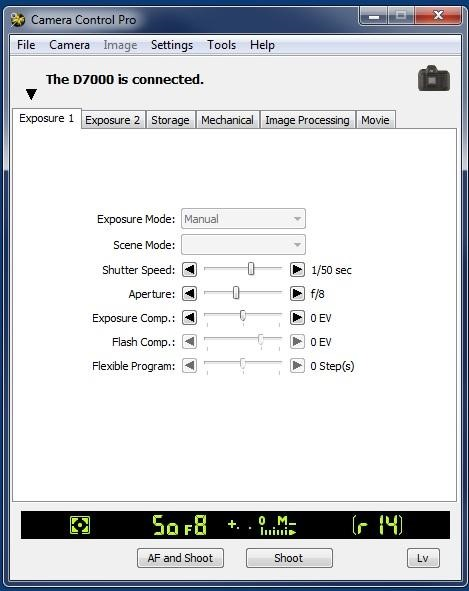
\includegraphics{images/Camera3.jpg}

\begin{itemize}
\item
  Click on ``\textbf{Exposure 2}'' under the Camera Control tabs and change the settings of the following:

  ISO Sensitivity: ISO 400\\
  White Balance: Auto\\
  Option: Normal
\end{itemize}

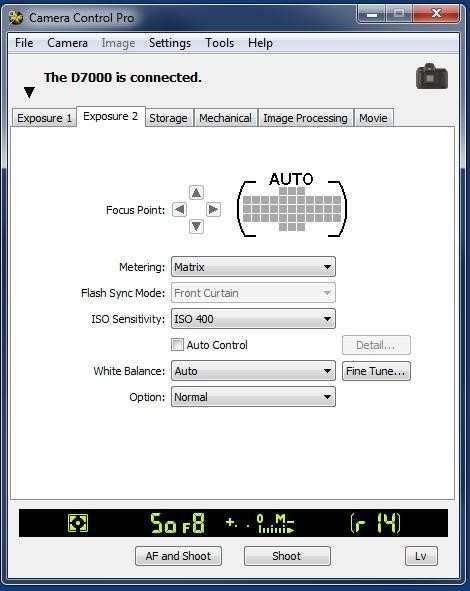
\includegraphics{images/Camera4.jpg}

\begin{itemize}
\item
  Click on ``\textbf{Storage}'' under the Camera Control tabs and change the settings of the following:

  Image Quality: JPEG fine\\
  JPEG Compression: Optimal quality\\
  Image size: Large (4928x3264)\\
  Record to: PC\\
  Card Record Mode: Backup
\end{itemize}

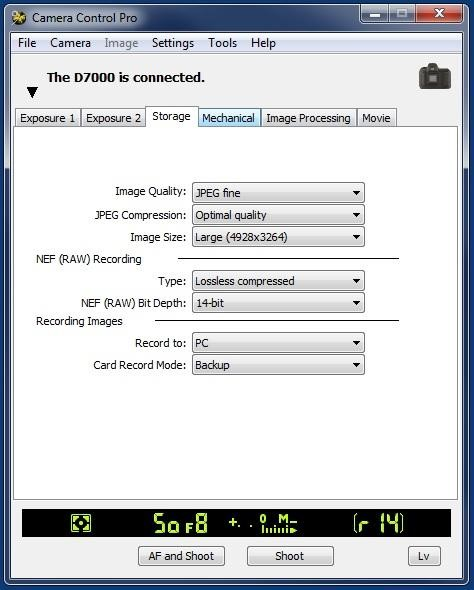
\includegraphics{images/Camera5.jpg}

\begin{itemize}
\item
  Click on ``\textbf{Image Processing}'' under the Camera Control tabs and change the settings of the following:

  Picture Control: Standard\\
  High ISO NR: On (High)
\end{itemize}

** \emph{Note: the above settings need to be set each time the software is reinstalled and the above settings will need to be modified if a new camera model/lens are used}

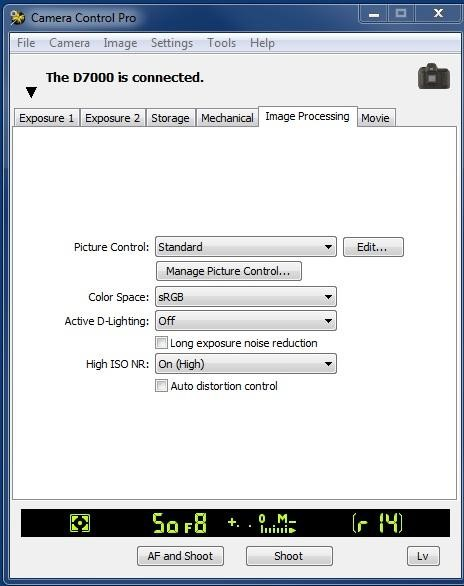
\includegraphics{images/Camera6.jpg}

\hypertarget{cau-plate-photo-documentation}{%
\subsubsection{CAU plate photo-documentation}\label{cau-plate-photo-documentation}}

\begin{enumerate}
\def\labelenumi{\arabic{enumi}.}
\tightlist
\item
  Ensure that the camera's Mode dial is set to ``M'' (Manual)
\end{enumerate}

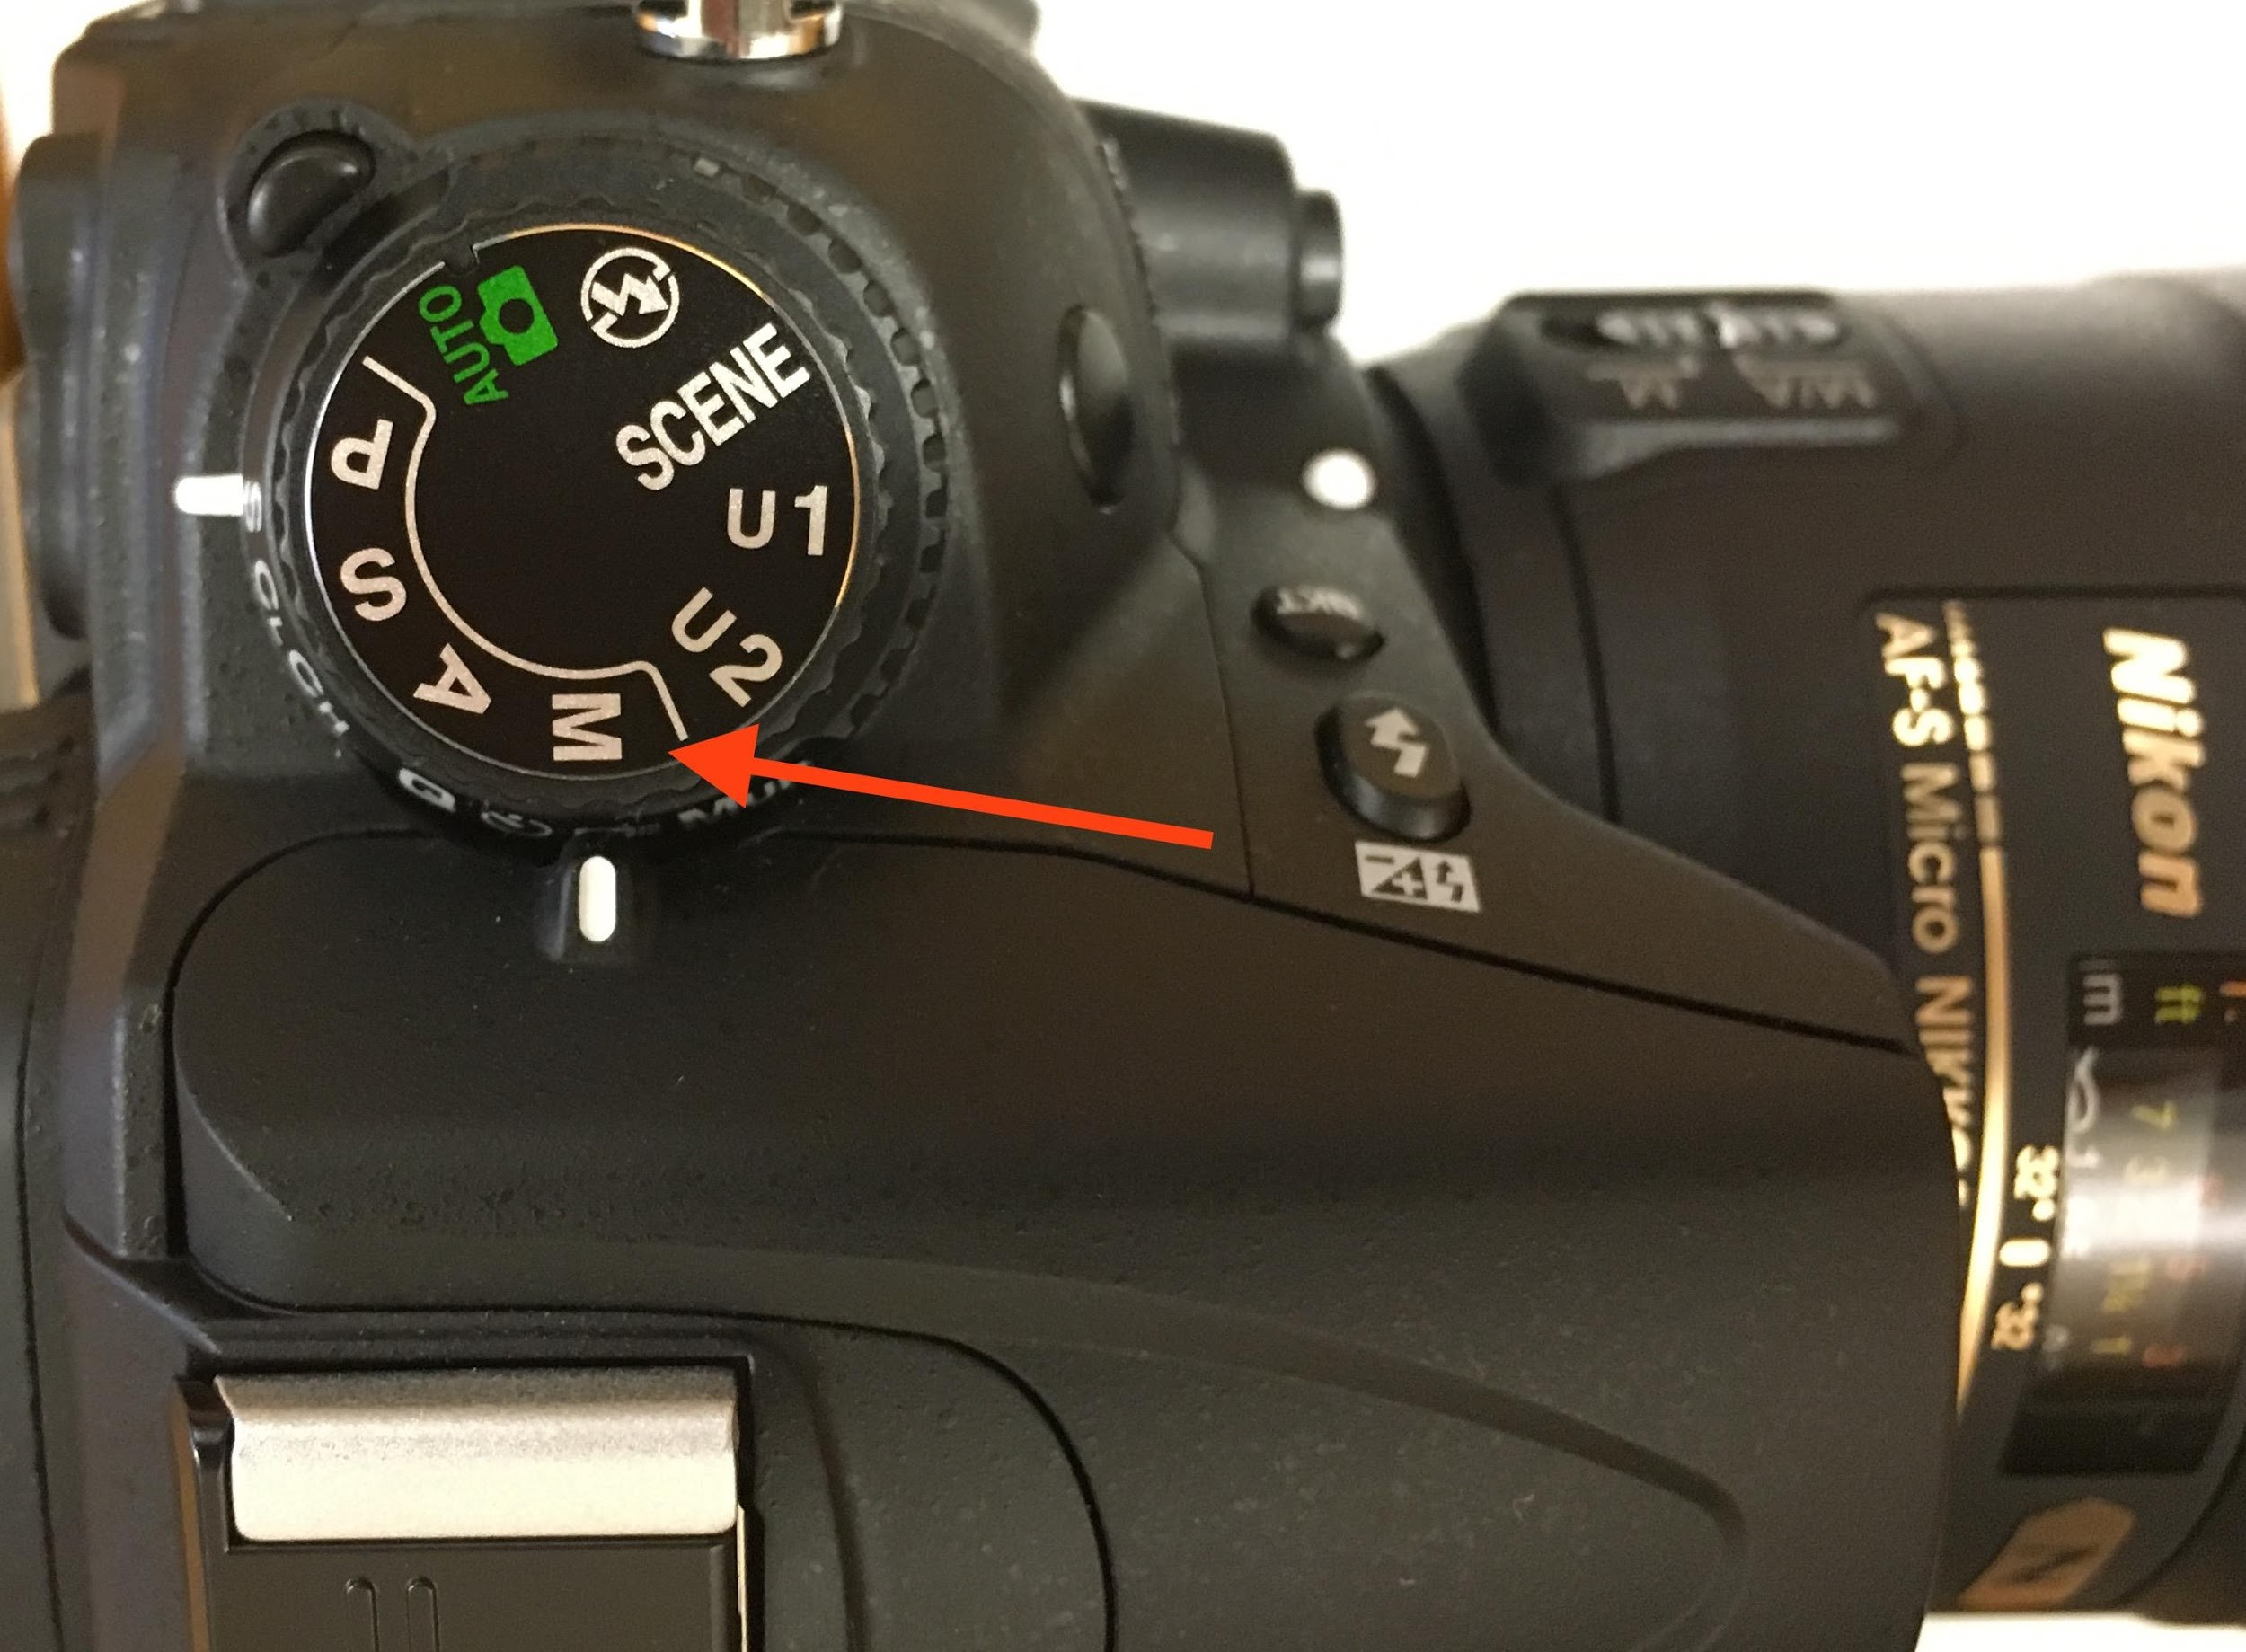
\includegraphics{images/Camera7.jpg}

\begin{enumerate}
\def\labelenumi{\arabic{enumi}.}
\setcounter{enumi}{1}
\tightlist
\item
  Ensure that the camera lens' A-M switch is set to ``M-A'' (Autofocus w/ manual override).
\end{enumerate}

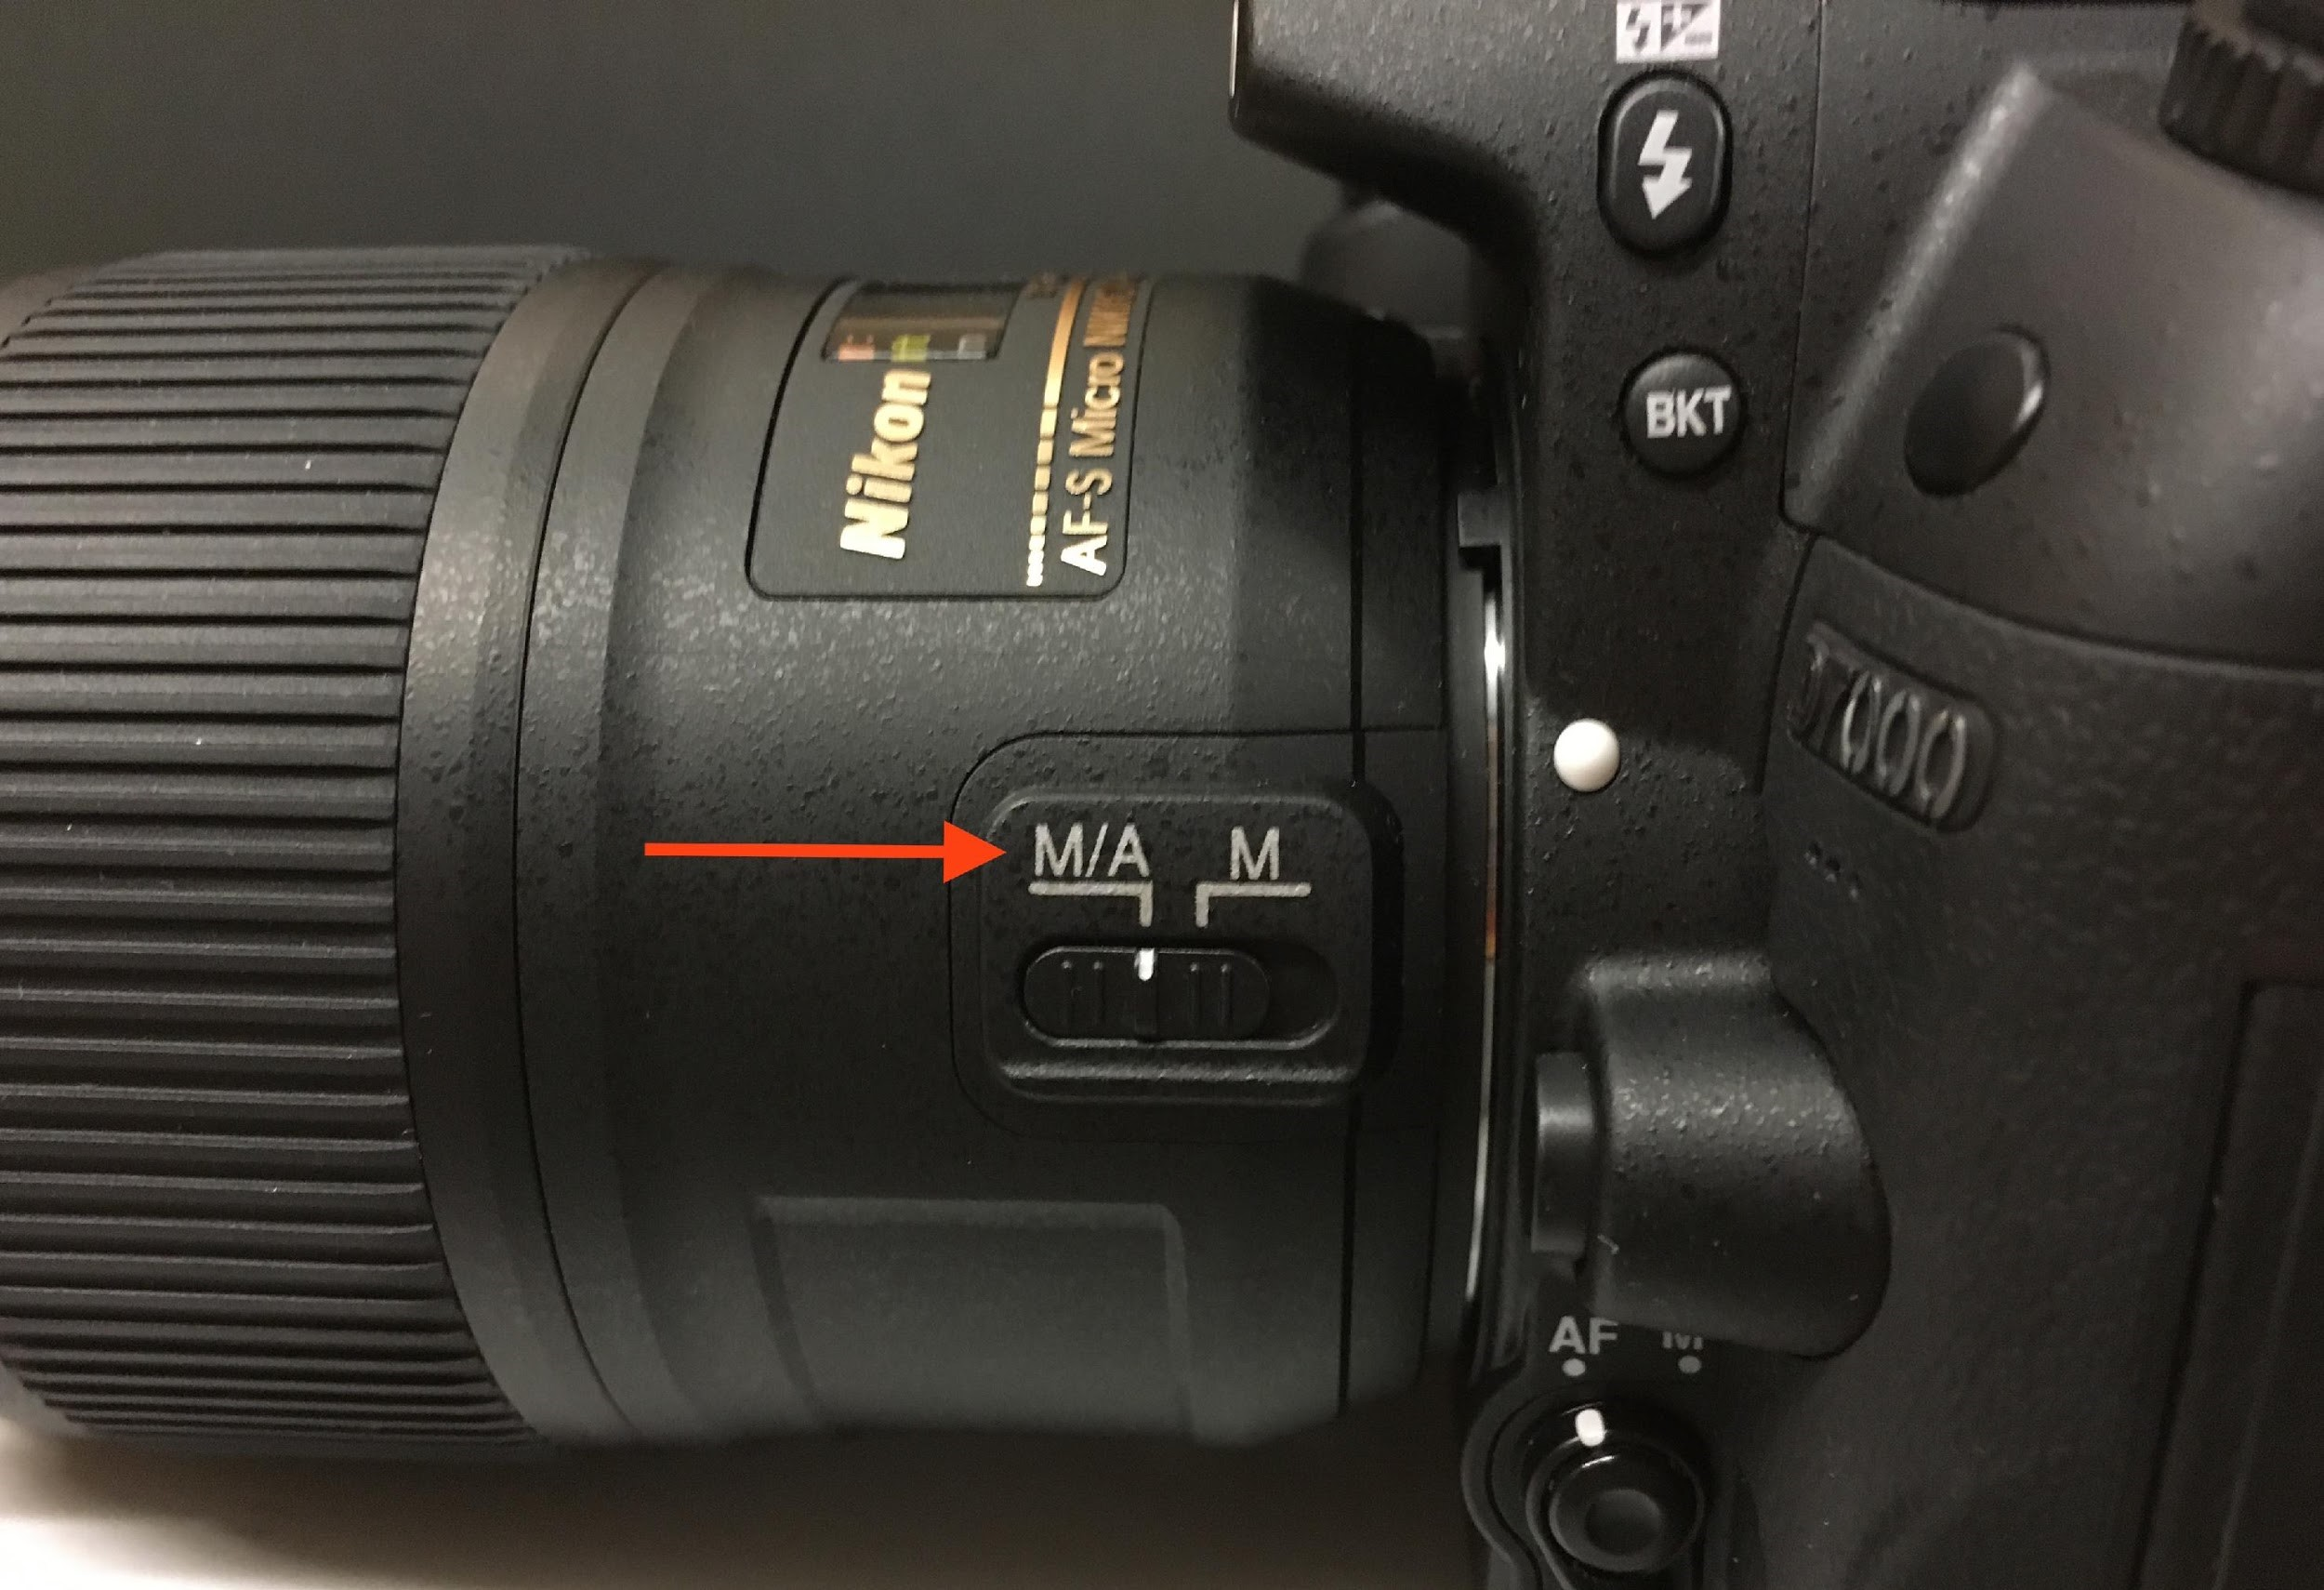
\includegraphics{images/Camera8.jpg}

\begin{enumerate}
\def\labelenumi{\arabic{enumi}.}
\setcounter{enumi}{2}
\tightlist
\item
  Connect the Nikon DSLR camera to the copier stand, then connect the camera to the computer via mini USB cable
\end{enumerate}

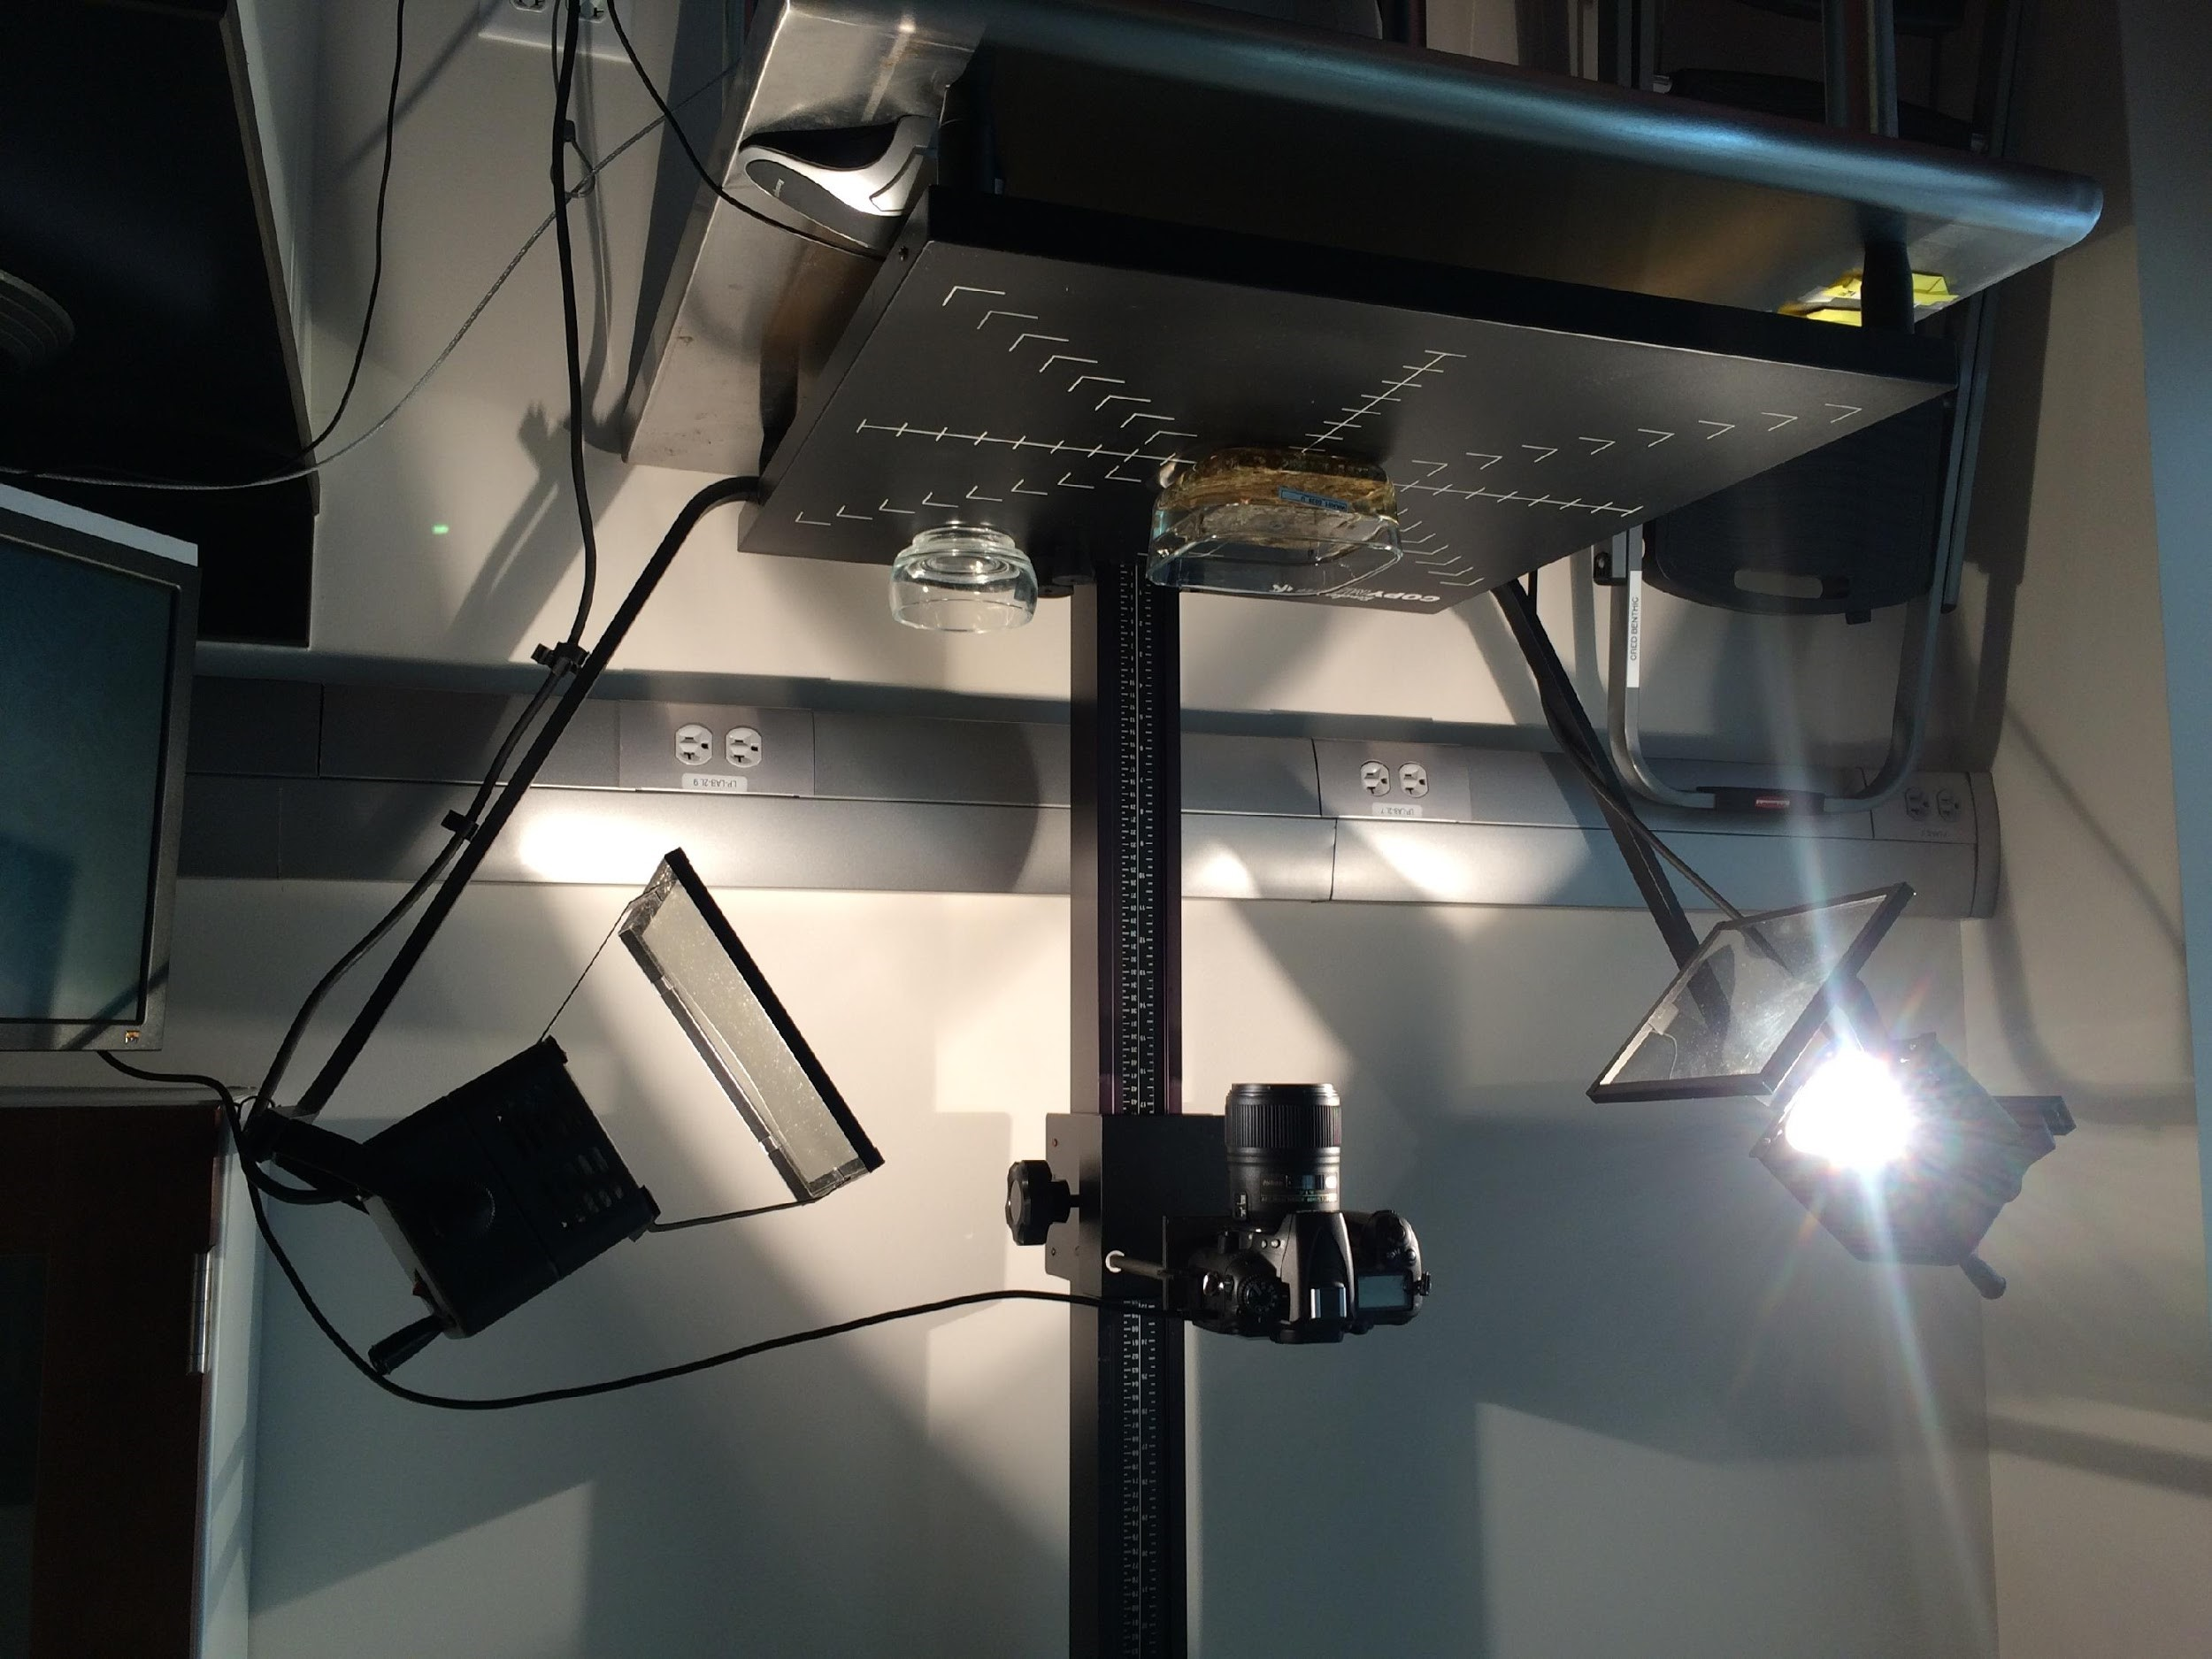
\includegraphics{images/Camera9.jpg}

\begin{enumerate}
\def\labelenumi{\arabic{enumi}.}
\setcounter{enumi}{3}
\item
  Start the Nikon Camera Control Pro 2 application
\item
  Turn the camera ON
\item
  Once connected, the connection status of the camera in use will be displayed on the Camera Control Pro main window
\end{enumerate}

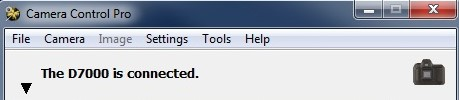
\includegraphics{images/Camera10.jpg}

\begin{enumerate}
\def\labelenumi{\arabic{enumi}.}
\setcounter{enumi}{6}
\tightlist
\item
  Go to the \textbf{Tools} menu to display the \textbf{Transfer Options} window
\end{enumerate}

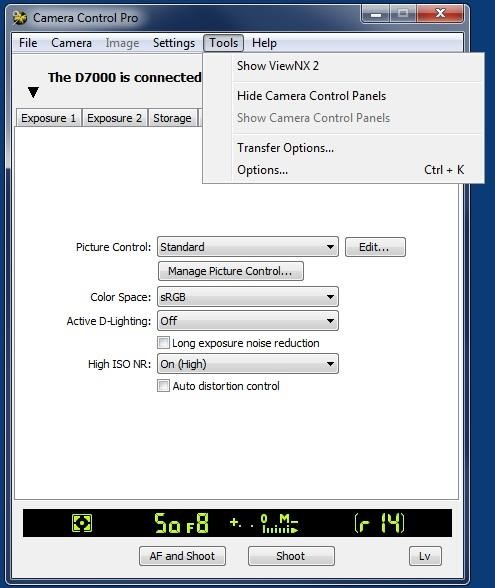
\includegraphics{images/Camera11.jpg}

\begin{enumerate}
\def\labelenumi{\arabic{enumi}.}
\setcounter{enumi}{7}
\item
  Click the \textbf{Browse} button next to the ``\emph{Destination folder}''. For ESD-CREP users, navigate to the appropriate CAU site and unit folder location

  ex: Documents\textbackslash CAU Analysis\textbackslash ASRAMP 2015\textbackslash PHOTO ANALYSIS\textbackslash SAMOA\textbackslash SWAINS\textbackslash SWA03\textbackslash SWA03\_368
\end{enumerate}

where the images will be downloaded as they are taken. Click \textbf{OK}

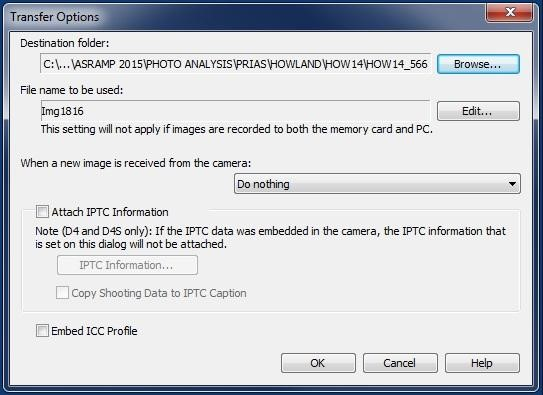
\includegraphics{images/Camera12.jpg}

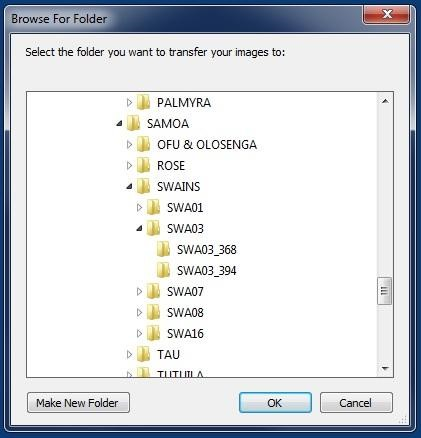
\includegraphics{images/Camera13.jpg}

\begin{enumerate}
\def\labelenumi{\arabic{enumi}.}
\setcounter{enumi}{8}
\tightlist
\item
  On the Camera Control Pro main window, click on the ``\textbf{LV}'' button at the bottom-right corner to display the Live View window.
\end{enumerate}

** \emph{Note: the camera controls and folder location options cannot be modified while the Live View window is displayed}

\includegraphics{images/Camera14.jpg}

\begin{enumerate}
\def\labelenumi{\arabic{enumi}.}
\setcounter{enumi}{9}
\tightlist
\item
  Center the glass dish with the plate under the camera and using the Live View display, ensure that all corners of the plate are visible in the frame
\end{enumerate}

** \emph{Note: both copier stand lights should be switched on at this time and that any external light sources are minimized (i.e., window shades are drawn, overhead/ceiling lights are switched off)}

\includegraphics{images/Camera15.jpg}

\begin{enumerate}
\def\labelenumi{\arabic{enumi}.}
\setcounter{enumi}{10}
\tightlist
\item
  Using the ``\textbf{AF and Shoot}'' button on the Live View window, photograph the top of the plate, \textbf{first with the Plate Photo ID tag} and then a \textbf{second image without the tag}
\end{enumerate}

\includegraphics{images/CAU_image.jpg}

\begin{enumerate}
\def\labelenumi{\arabic{enumi}.}
\setcounter{enumi}{11}
\item
  Flip the plate and photograph the \textbf{bottom} of the plate, again with Plate Photo ID tag and then a second image without the tag
\item
  From the designated CAU unit folder, confirm that both plate photos (with and without the Plate Photo ID tag) are in focus
\item
  Repeat for the next set of plates/surfaces for each unit
\item
  After all 8 images have been taken and saved to the unit folder (e.g.~SWA03\_368), click on the ``\textbf{LV}'' button at the bottom-right corner to turn off Live View
\item
  On the Camera Control Pro main window, go to the Tools menu to display the \textbf{Transfer Options window}. Click on the \textbf{Browse} button next to the ``\emph{Destination folder}'' and \textbf{navigate to the next CAU site and unit folder} (e.g.~\emph{SWA03\_394}). Repeat steps C. 7-13
\end{enumerate}

\includegraphics{images/Camera16.jpg}

\includegraphics{images/Camera17.jpg}

\begin{enumerate}
\def\labelenumi{\arabic{enumi}.}
\setcounter{enumi}{16}
\item
  At the end of the plate photo documentation session, ensure that all CAU plate photos have been taken and saved to their appropriate local drive folders
\item
  Backup the images by copying the \textbf{Island} parent folder,

  ex: Documents-CAU Analysis-ASRAMP 2015-PHOTO ANALYSIS-SAMOA-SWAINS
\end{enumerate}

to the network drive,

\begin{verbatim}
ex: T:\\Oceanography\\CAUs\\Analysis\\2018_CAU Analysis\\ASRAMP18\\PHOTO ANALYSIS\\SAMOA\\SWAINS   
\end{verbatim}

and to the external hard drive. If prompted, select ``Overwrite''

\begin{enumerate}
\def\labelenumi{\arabic{enumi}.}
\setcounter{enumi}{18}
\item
  Turn off the camera and disconnect it from the mini USB cable. On the Camera Control Pro main window, select Exit from the File menu
\item
  Rename all plate photos with the following naming convention:
\end{enumerate}

\begin{itemize}
\item
  \textbf{With Plate Photo ID tag:}\\
  *SiteID\_RecoveryYear\_4-digitSerial\#\_PlateLocation (``U'' - upper plate or ``L'' - lower plate)\_PlateSurface (``T'' - top plate or ``B'' - bottom plate)\_ID.jpg*
\item
  \textbf{Without Plate Photo ID tag:}\\
  *SiteID\_RecoveryYear\_4-digitSerial\#\_PlateLocation (``U'' - upper plate, ``L'' - lower plate)\_PlateSurface (``T'' - top plate, ``B'' - bottom plate).jpg*

  Example:
  PAL01\_2012\_5319\_U\_T\_ID.jpg -- Upper Plate, Top Side with tag\\
  PAL01\_2012\_5319\_U\_T.jpg -- Upper Plate, Top Side\\
  PAL01\_2012\_5319\_U\_B\_ID.jpg -- Upper Plate, Bottom Side with tag
  PAL01\_2012\_5319\_U\_B.jpg -- Upper Plate, Bottom Side\\
  PAL01\_2012\_5319\_L\_T\_ID.jpg -- Lower Plate, Top Side with tag\\
  PAL01\_2012\_5319\_L\_T.jpg -- Lower Plate, Top Side\\
  PAL01\_2012\_5319\_L\_B\_ID.jpg -- Lower Plate, Bottom Side with tag\\
  PAL01\_2012\_5319\_L\_B.jpg -- Lower Plate, Bottom Side
\end{itemize}

\includegraphics{images/Camera18.jpg}

\begin{enumerate}
\def\labelenumi{\arabic{enumi}.}
\setcounter{enumi}{20}
\item
  Copy the newly-renamed images to the network folder by copying the \textbf{Island} parent folder

  e.g.~Documents-CAU Analysis-ASRAMP 2015-PHOTO ANALYSIS-SAMOA-SWAINS
\end{enumerate}

to the network drive

\begin{verbatim}
e.g. T:\\Oceanography\\CAUs\\Analysis\\2018_CAU Analysis\\ASRAMP18\\PHOTO ANALYSIS\\SAMOA\\SWAINS  
\end{verbatim}

and to the external hard drive. If prompted, select ``Overwrite''

\hypertarget{postcruise}{%
\chapter{Post Cruise Activities}\label{postcruise}}

\hypertarget{data-qc-and-import-into-oracle-database}{%
\section{Data QC and Import into Oracle Database}\label{data-qc-and-import-into-oracle-database}}

\hypertarget{instrument-refurbishment}{%
\section{Instrument Refurbishment}\label{instrument-refurbishment}}

\hypertarget{this-is-an-example-blank-chapter}{%
\chapter{This is an Example Blank Chapter}\label{this-is-an-example-blank-chapter}}

copy it and use it as a template if you like

This is how you insert an image:
\includegraphics{images/OCC_Diurnal_Suite_Recovery_CJS.jpg}


\end{document}
